
\chapter{System Design}
\label{ch:system_design}

\begin{figure}[H]
    \centering
    
\includegraphics[width=0.75\textwidth]{images/Section_5/Full_Arch.png}
    \caption{System Architecture Diagram}
    \label{fig:system_architecture}
\end{figure}
\restoregeometry

This section first introduces the overall design of the system, followed by a detailed breakdown of its main modules.

The design aims to satisfy the FRs defined in Chapter~\ref{ch:requirements} while maintaining a balance between system modularity and implementation complexity.

Figure~\ref{fig:system_architecture} illustrates the high-level system architecture. The system employs a \textbf{layered design}, consisting of a frontend, API gateway, backend services, AI models, and data storage components. 
This layered structure is chosen instead of a microservices-based architecture because it provides a clear separation of different components, and for projects of this scale, implementation and management are simpler.

Users interact with the system through a frontend interface, which provides core functionalities such as recommendations based on LLMs, virtual try-on, wardrobe management, scheduling, and wardrobe analysis. Then, all user requests are first processed by the API gateway, which serves as a unified entry point, routing the requests to the corresponding backend services. The backend is organized into multiple service modules, including LLM services, image processing services, and user-related services. 

This modular organization is adopted to separate different types of processing logic and reduce coupling between components, making the system easier to maintain and extend. 

Based on this overall architecture, the following sections will provide a detailed description of each module.

\section{Module Decomposition}

\subsection{Front-end Module}
\begin{figure}[h]
    \centering
    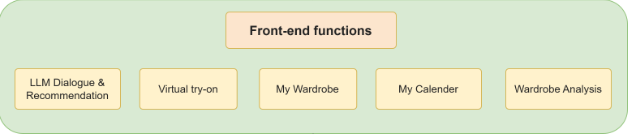
\includegraphics[width=0.8\textwidth]{images/Section_5/Frontend.png}
    \caption{Front-end Module}
    \label{fig:frontend_module}
\end{figure}

As shown in Figure \ref{fig:frontend_module}, the front-end module is designed as an interaction layer, focusing on user experience and request orchestration rather than computation processing. All complex logic, including recommendation generation, image processing, and data analysis, is delegated to backend services through an API gateway. This module therefore serves as the entry point of the system, enabling users to interact with various intelligent functions through an intuitive and unified interface.

In this module, since organizing the system by user workflow is more intuitive than splitting it by technical components, we also divided the interface into five independent user interface components. Each component encapsulates a complete user workflow, enhancing the degree of modularity and allowing for independent development, testing, and future expansion.

\begin{enumerate}
    \item \textbf{LLM Dialogue UI} - accepts natural language queries or refinement instructions from users
    \item \textbf{Virtual try-on UI} - renders generated preview and supports re-tries or saving 
    \item \textbf{My Wardrobe UI} -  supports upload, organize, search, filter, and virtually try-on clothing items.
    \item \textbf{My Calendar UI} - lets users track daily looks, review monthly styling activity, and add outfits to specific dates.
    \item \textbf{Wardrobe Analysis UI} - helps users track clothing usage, identify unworn items, view category distribution, and receive smart recommendations for wardrobe additions.
\end{enumerate}



\subsection{Back-end Module (Core Services)}

\begin{figure}[H]
    \centering
    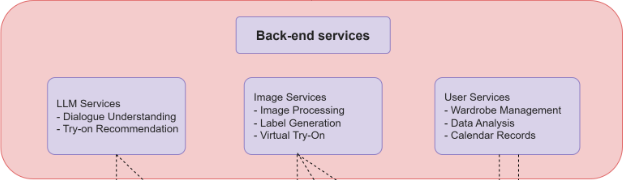
\includegraphics[width=0.8\textwidth]{images/Section_5/Backend.png}
    \caption{Back-end Module (Core Services)}
    \label{fig:backend_module}
\end{figure}

The back-end implements business logic and orchestrates data flow. Exposes REST endpoints via \textbf{FastAPI}, serving as the single point of interaction between the front-end and the AI model layer.

\vspace{0.5cm}
\textbf{\large (1) LLM Services Responsibilities}

\textbf{Design Motivation} 

The LLM service module aims to handle dialogue understanding and recommendation generation based on user input. Since user requests are expressed in natural language and may contain implicit preferences, a dedicated module is required to interpret user intent and convert it into structured output to support downstream tasks, such as clothing recommendation and virtual try-on.

\textbf{Module Design} 

This module processes user queries and dialog contexts to extract semantic constraints such as style, occasion, and preference. Then, it generates recommendation-oriented outputs, including outfit suggestions, candidate products, and reasoning texts. These outputs are structured and can be directly used by the frontend or passed to other services, such as image-based try-on.

\textbf{Input/Output}\\[0.3cm]
\textbf{IN:} user text, behavior history, wardrobe metadata\\[0.2cm]
\textbf{OUT:} outfit descriptions, item candidates, reasoning text, retrieval tags

This design integrates language understanding and recommendation functions into a single module, enhancing the degree of modularity and facilitating interaction with other services.

\vspace{0.5cm}

\textbf{\large (2) Image Services Responsibilities}

\textbf{Design Motivation} 

The design of this module is motivated by the need to convert \textbf{raw clothing images} into \textbf{structured and usable information} for the overall system. Since uploaded garment images are inherently unstructured, they cannot be directly consumed by downstream components such as recommendation, retrieval, and virtual try-on. Therefore, a dedicated image-related module is needed to bridge the gap between low-level visual input and high-level semantic understanding. 

This module allows the system to process clothing images in a consistent way and provide standardized outputs for different back-end services.

\textbf{Module Design} 

Based on this motivation, the module is designed to integrate \textbf{semantic extraction}, \textbf{attribute labeling}, and \textbf{image preprocessing} into a unified pipeline. It is responsible for \textbf{extracting semantic representations} from clothing images and generating corresponding \textbf{attribute labels}, such as \textbf{color}, \textbf{category}, and \textbf{aesthetic style}, so that clothing items can be better understood, indexed, and managed by the system. In addition, the module performs \textbf{normalization and preprocessing} on raw images to improve input consistency and support more reliable downstream analysis. It also supports \textbf{asset preparation for virtual try-on}, ensuring that clothing resources are properly formatted and organized for subsequent synthesis tasks.


\textbf{Interaction Flow}\\
Receives images $\rightarrow$ invoke model $\rightarrow$ stores extracted embeddings/labels

Overall, this design keeps image-related processing in a unified pipeline rather than distributing it across different modules, which reduces redundancy, ensures consistent data formats, and improves the reliability of downstream AI services.

\vspace{0.5cm}

\textbf{\large (3) User Services}
\textbf{Responsibility}

\textbf{Design Motivation} 

The \textbf{User Services} module is designed to centralize the management of wardrobe data, user records, and analytical information within the system. Since recommendation, retrieval, and calendar-based outfit tracking all rely on consistent and well-organized user data, a dedicated service layer is needed to coordinate these operations.

\textbf{Module Design} 

The \textbf{User Services} module is responsible for \textbf{wardrobe management}, \textbf{data analysis}, and \textbf{calendar records}. It manages the overall structure of the user's wardrobe, supports item-related operations, and provides filtered clothing information for downstream tasks such as recommendation and retrieval. It also stores user-related metadata and outfit records, which can be used for usage analysis, profile construction, and personalized recommendation. In addition, this service layer guarantees that the model modules never directly \textbf{read from} or \textbf{write to} the data layer, which helps maintain clear system boundaries and improves modularity and maintainability.

By centralizing user-related data in a dedicated service layer, the system avoids direct data access from model components and reduces duplication across modules. This helps maintain consistent data structures and clearer boundaries, making the system easier to maintain and extend.

\subsection{AI Model Layer}
\begin{figure}[h]
    \centering
    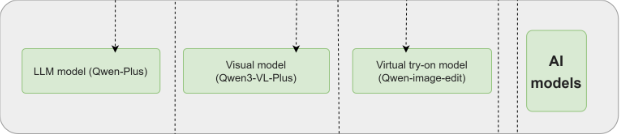
\includegraphics[width=0.8\textwidth]{images/Section_5/AI_models.png}
    \caption{AI Model Layer}
    \label{fig:ai_model_layer}
\end{figure}

This layer performs heavy computation tasks and is stateless from the system's perspective. To avoid coupling model execution with application logic, we isolate AI models into a separate layer rather than embedding them directly into backend services.

Under this design, backend services invoke specialized model APIs, where different models work together to mimic the reasoning process of human designers. This modular approach abstracts complex execution logic from the core system, aligns with recent agent architectures based on LLMs \citep{xi2023llm_agents}, and follows the design principles of scalable distributed systems for deep learning inference \citep{dragoni2016microservices}.

\vspace{0.5em}
\noindent\textbf{(1) Qwen-Plus (Dialogue Understanding \& Recommendation).}

A primary challenge in fashion recommendation is bridging the semantic gap between a user's abstract, conversational needs and the database's strict taxonomy. Rather than forcing users to navigate complex filter menus, Qwen-Plus acts as a semantic translation layer. It is used for understanding dialog, generating recommendations, and preparing structured output. It interprets unstructured user requests, applies aesthetic reasoning, and translates natural language into outfit suggestions and structured tags that align with the system's predefined taxonomy. 

\vspace{0.5em}
\noindent\textbf{(2) Qwen-VL-Plus (Visual Perception \& Tagging).}

To minimize the friction of manual digital wardrobe management, the system required an automated perception mechanism. We implemented Qwen-VL-Plus for per-item representation learning, semantic label extraction, and category and pairing inference. It analyzes individual clothing images and autonomously extracts granular descriptive labels (category, color, material), while also inferring potential matching relationships. By offloading the tagging burden from the user to a Vision-Language Model, we ensure the database is populated with standardized, high-quality metadata, which supports efficient retrieval and downstream reasoning.

\vspace{0.5em}
\noindent\textbf{(3) Qwen-Image-Edit (Virtual Try-On Synthesis).}

The effectiveness of virtual try-on mainly depends on visual fidelity. During development, we found that baseline models often over-apply masks, which will distort the user’s pose or details.

Therefore, we chose Qwen-Image-Edit to prioritize output quality and identity consistency, even though this makes deployment more complex and increases computational cost. This model is used for virtual try-on tasks, such as person-clothing synthesis and clothing replacement, and it takes predefined prompts and image inputs to generate consistent images. This ensures that the try-on results presented by the system have stronger visual realism and fewer artifacts, while retaining the user's local physical features and lighting environment as a reliable validation step for styling decisions.


\subsection{Data Layer}
\begin{figure}[H]
    \centering
    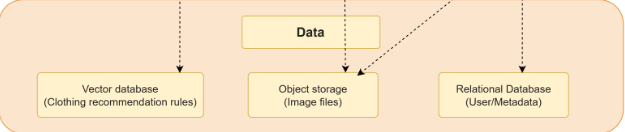
\includegraphics[width=0.8\textwidth]{images/Section_5/Data.png}
    \caption{Data Layer}
    \label{fig:data_layer}
\end{figure}

\textbf{\large Object Storage}\\[0.2cm]
The \textbf{object storage} is used to store raw image assets, including original wardrobe uploads, virtual try-on preview images, and historical generated outputs. The back-end maintains only URIs or corresponding metadata rather than storing image directly. This approach improves scalability and ensures storage independence from application logic.\\

\textbf{\large Relational Database}\\[0.2cm] 
The \textbf{relational database} stores structured entities such as user accounts, clothing metadata, tags and attributes, and usage statistics. A relational schema provides predictable retrieval and analytical querying capabilities, while preventing excessive load on the embedding layer and avoiding semantic ambiguity.\\

\textbf{\large Vector Database}\\[0.2cm]
The \textbf{vector database} is designed to store semantic representations of \textbf{clothing recommendation rules} and related fashion knowledge. It allows the system to retrieve relevant matching guidance, style patterns, and recommendation constraints based on semantic similarity, rather than relying only on exact text matching. In this way, the database supports more context-aware and personalized recommendation generation.

\newpage




\section{Key User–Service Interactions (Sequence Diagrams)}
\textbf{\large 1. Virtual Try-on Sequence\\ (corresponding to UC-05 Virtual Try-on)}
\begin{figure}[H]
    \centering
    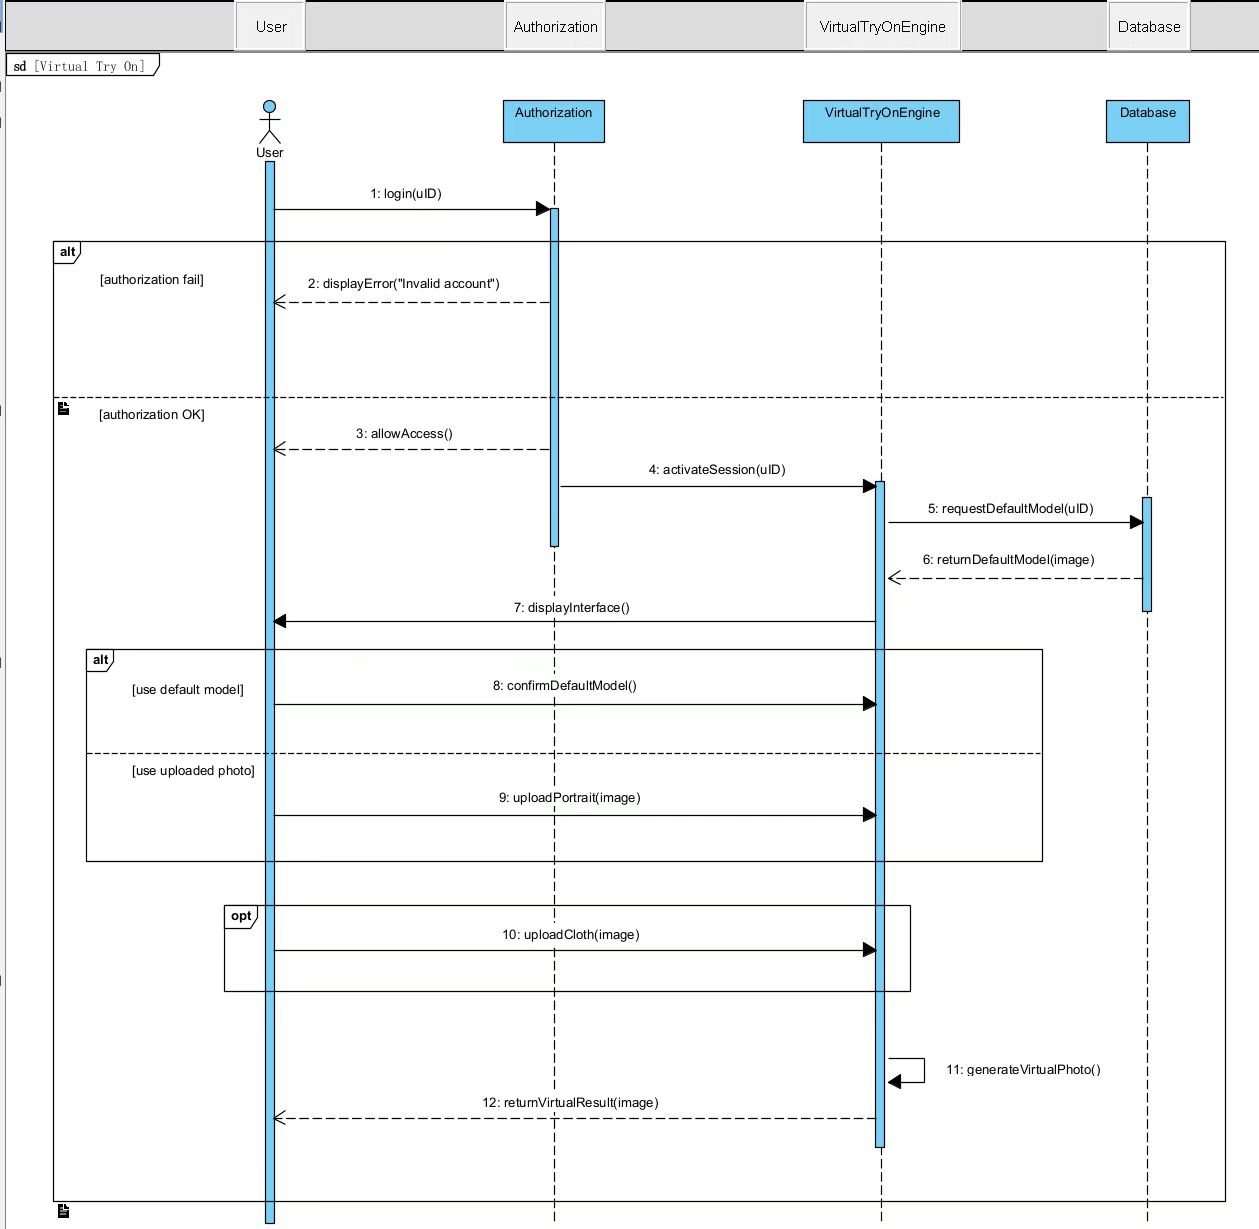
\includegraphics[width=1\textwidth]{images/Section_5/Sequence/Try_on.jpg}
    \caption{Virtual Try-on sequence diagram}
    \label{fig:Virtual try-on}
\end{figure}

\textbf{Justification \& link to requirements}\\
This sequence diagram illustrates that the try-on engine is encapsulated in the backend service, and the front end only sends images and parameters without directly interacting with the model.

It supports the virtual try-on of user photos (FR-10) and the virtual try-on of clothing images (FR-11), and connects with the subsequent process of exporting and sharing the try-on results (FR-12).\\


\textbf{\large 2. LLM Recommendation Sequence\\ (corresponding to UC-03 Get Outfit Recommendation \& UC-04 Provide Feedback) }
\begin{figure}[H]
    \centering
    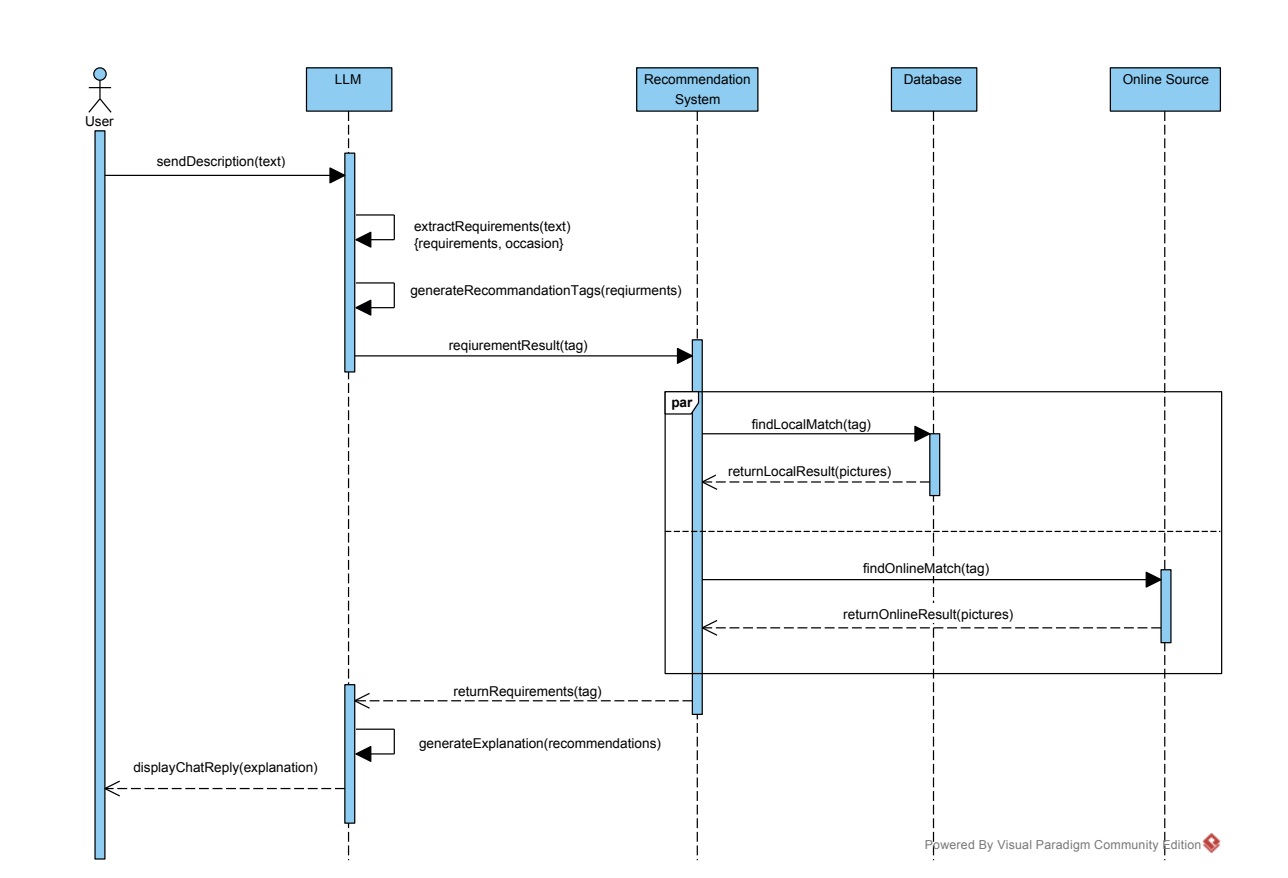
\includegraphics[width=1\textwidth]{images/Section_5/Sequence/Recommend.png}
    \caption{LLM Recommendation sequence diagram}
    \label{fig:Recommend}
\end{figure}

\textbf{Justification \& link to requirements}\\
This sequence diagram demonstrates the consistency between the recommendation process and the high-level architecture: front-end conversation → LLM service → recommendation system → data layer/external resources, and then back to the user interface, without any layer-over-layer access. 

It implements FR-04 user preference profiling, FR-05 input of occasion and constraints, FR-06 weather data acquisition, FR-07 outfit recommendation, and FR-08 recommendation explanation and alternative options; combined with the subsequent user feedback process, it also provides interfaces for FR-09 feedback loop and learning.\\


\newpage
\textbf{\large 3. Wardrobe Management Sequence\\ (Corresponding to UC-02 Manage Digital Wardrobe) }
\begin{figure}[H]
    \centering
    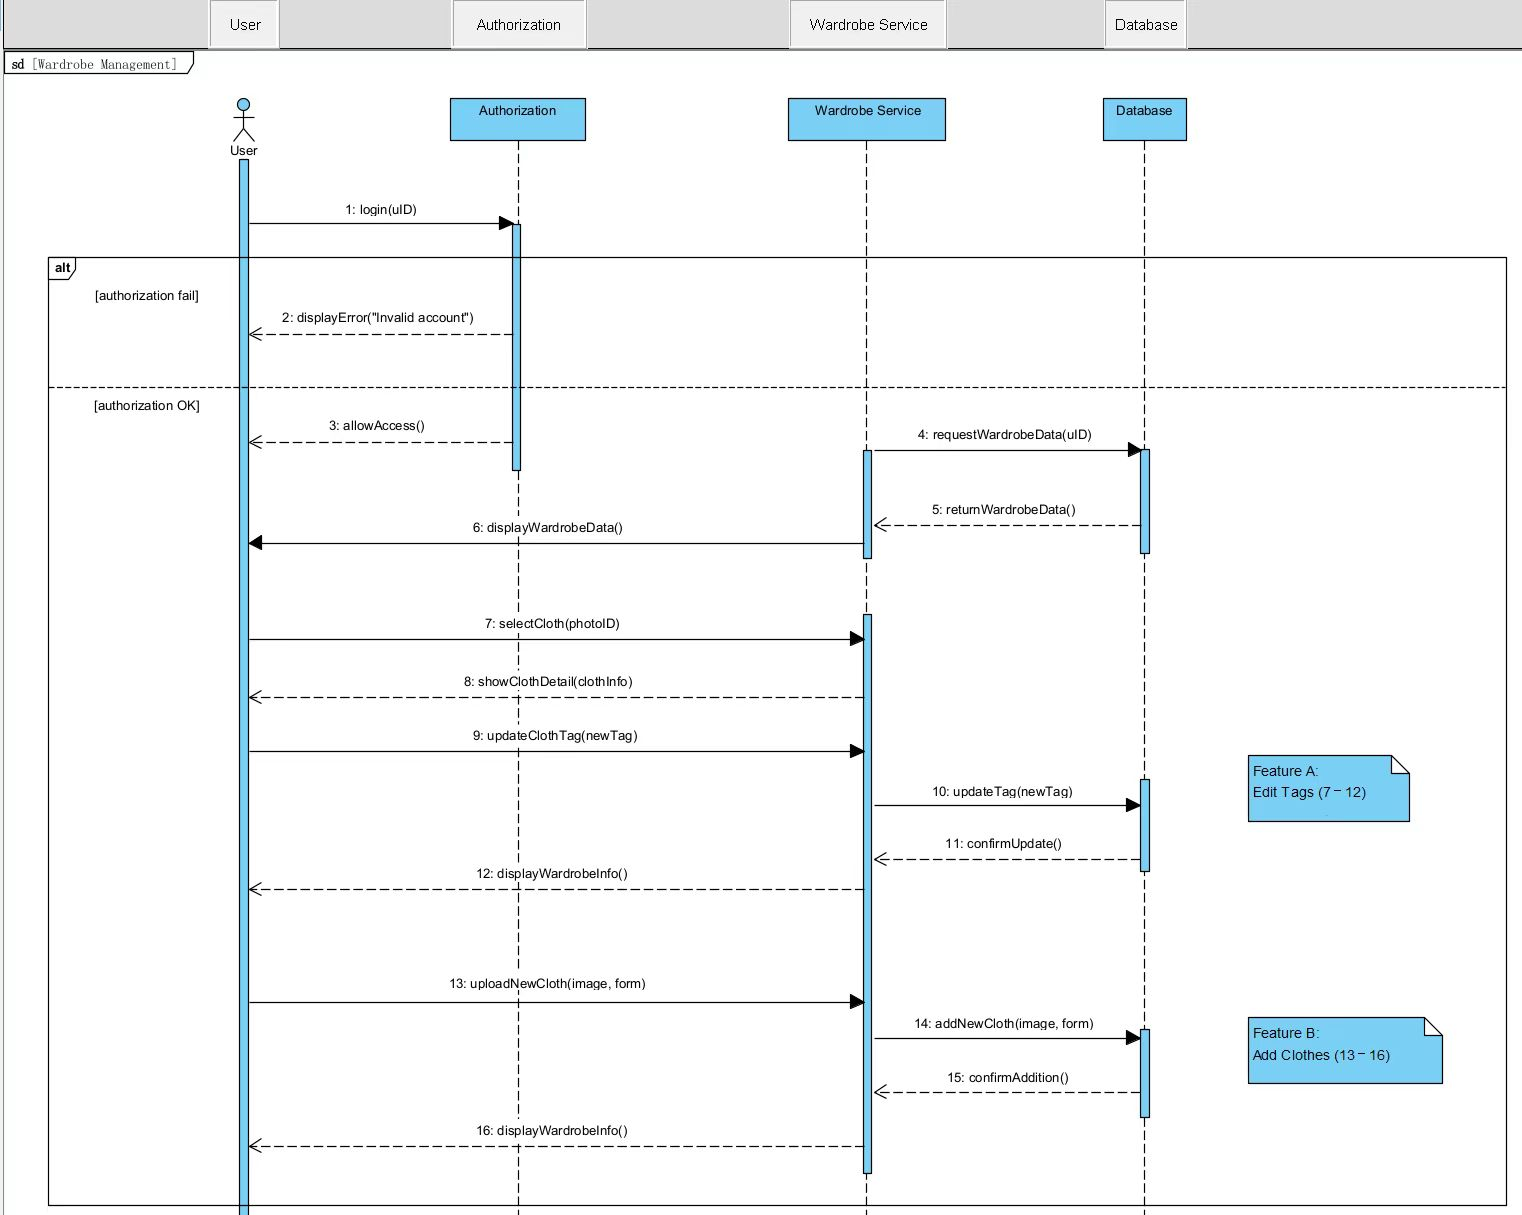
\includegraphics[width=1\textwidth]{images/Section_5/Sequence/Wardrobe_manage.jpg}
    \caption{Wardrobe Management sequence diagram}
    \label{fig:Wardrobe_management}
\end{figure}

\textbf{Justification \& link to requirements}\\
This sequence diagram illustrates the design where the front end accesses the data layer only through the service layer. 

It directly implements FR-01 account login, FR-02/FR-03 wardrobe creation (forms and images), and FR-13 wardrobe maintenance (query, filtering, batch editing), proving that the core wardrobe management function is feasible at the system level.\\


\newpage
\textbf{\large 4. Wardrobe Analysis Sequence\\ (Corresponding to UC-07 View/Edit User Profile)}
\begin{figure}[H]
    \centering
    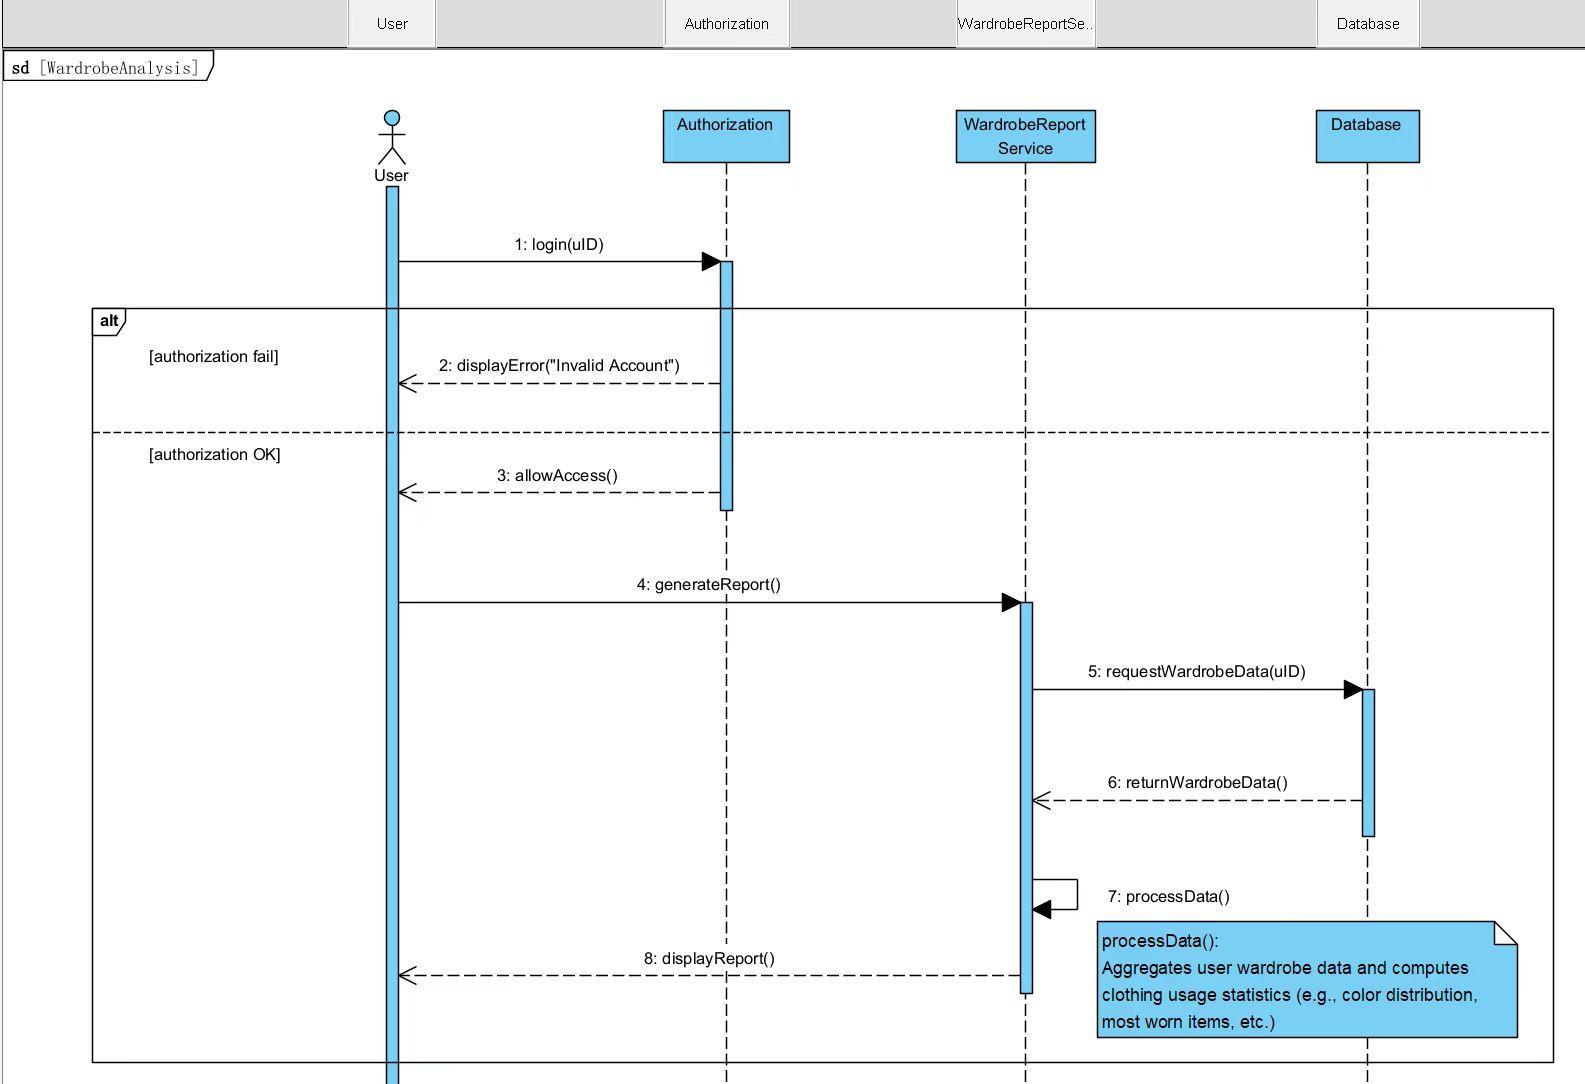
\includegraphics[width=1\textwidth]{images/Section_5/Sequence/Wardrobe_analysis.jpg}
    \caption{Wardrobe Analysis sequence diagram}
    \label{fig:Wardrobe_analysis}
\end{figure}

\textbf{Justification \& link to requirements}\\
This sequence diagram illustrates that preference profile is accomplished through independent analysis services, decoupled from ordinary CRUD operations. 

It realizes and supports the requirements for historical records and statistical views in FR-04 User Preferences (Profile Generation and Display) and FR-13 Wardrobe Maintenance, providing a data foundation for subsequent recommendations and visual analysis.\\

\newpage

\section{Database Schema and Storage Structure}
We design a relational database schema (PostgreSQL) to support structured wardrobe data management. The schema is centered around several core entities: 
\begin{itemize}
    \item The \textbf{Users} table manages authentication and profile information. 
    \item \textbf{Clothing Items} store individual wardrobe entries, linked to users via foreign keys.
    \item \textbf{Outfits} represent combinations of clothing items, enabling recommendation and reuse.
    \item \textbf{Wear History} records user interactions with clothing and outfits over time, supporting analytics and personalization.
\end{itemize}

These entities are connected through foreign key relationships, allowing efficient querying of user-specific wardrobe data and enabling features such as recommendation, tracking, and virtual try-on.

The detailed database schema, including all attributes and data types, is provided in Appendix \ref{database_schema}.



\section{UI Design}
\label{chapter_ui_design}
The UI of our project is designed with both functional requirements and non-functional requirements, aiming to provide a clear and efficient user interaction experience.

Functionally, the interface is organized around the core modules of the system, including user authentication (FR-01), wardrobe management (FR-02, FR-13), recommendation system (FR-05 - FR-09) and virtual try-on (FR-10 – FR-12). These features are implemented across different pages and integrated through a consistent design, allowing users to smoothly complete the workflow, from providing clothes to receiving recommendations.

From a non-functional perspective, our UI also considers usability and consistency. For example, Key tasks such as uploading clothing or obtaining recommendations are supported by simplified interaction flows, allowing users to complete them in a small number of steps, thereby satisfying the usability requirement (NF-05). In addition, the interface follows a consistent design style (NF-04), including colors, layout, and component structure, to improve the overall user experience. 


\subsection{Visual theme}
As shown in Fig.\ref{fig:ui_login}, the overall interface adopts a warm color combination of cream and warm brown. The background is a light grayish beige, while the main buttons and titles are highlighted in a darker warm brown and caramel color. This consistent use of colors and visual elements follows NF-04, ensuring a unified design across all pages.

We were inspired by the colors of traditional wooden closets, and aim to create a gentle and non-distracting visual atmosphere, while reducing the coldness of the software as a tool.

\begin{figure}[H]
    \centering
    % 左图
    \begin{minipage}[b]{0.48\textwidth}
        \centering
        
\includegraphics[width=\textwidth]{images/Section_5/newUI/login.png}
    \end{minipage}
    \hfill
    % 右图
    \begin{minipage}[b]{0.48\textwidth}
        \centering
        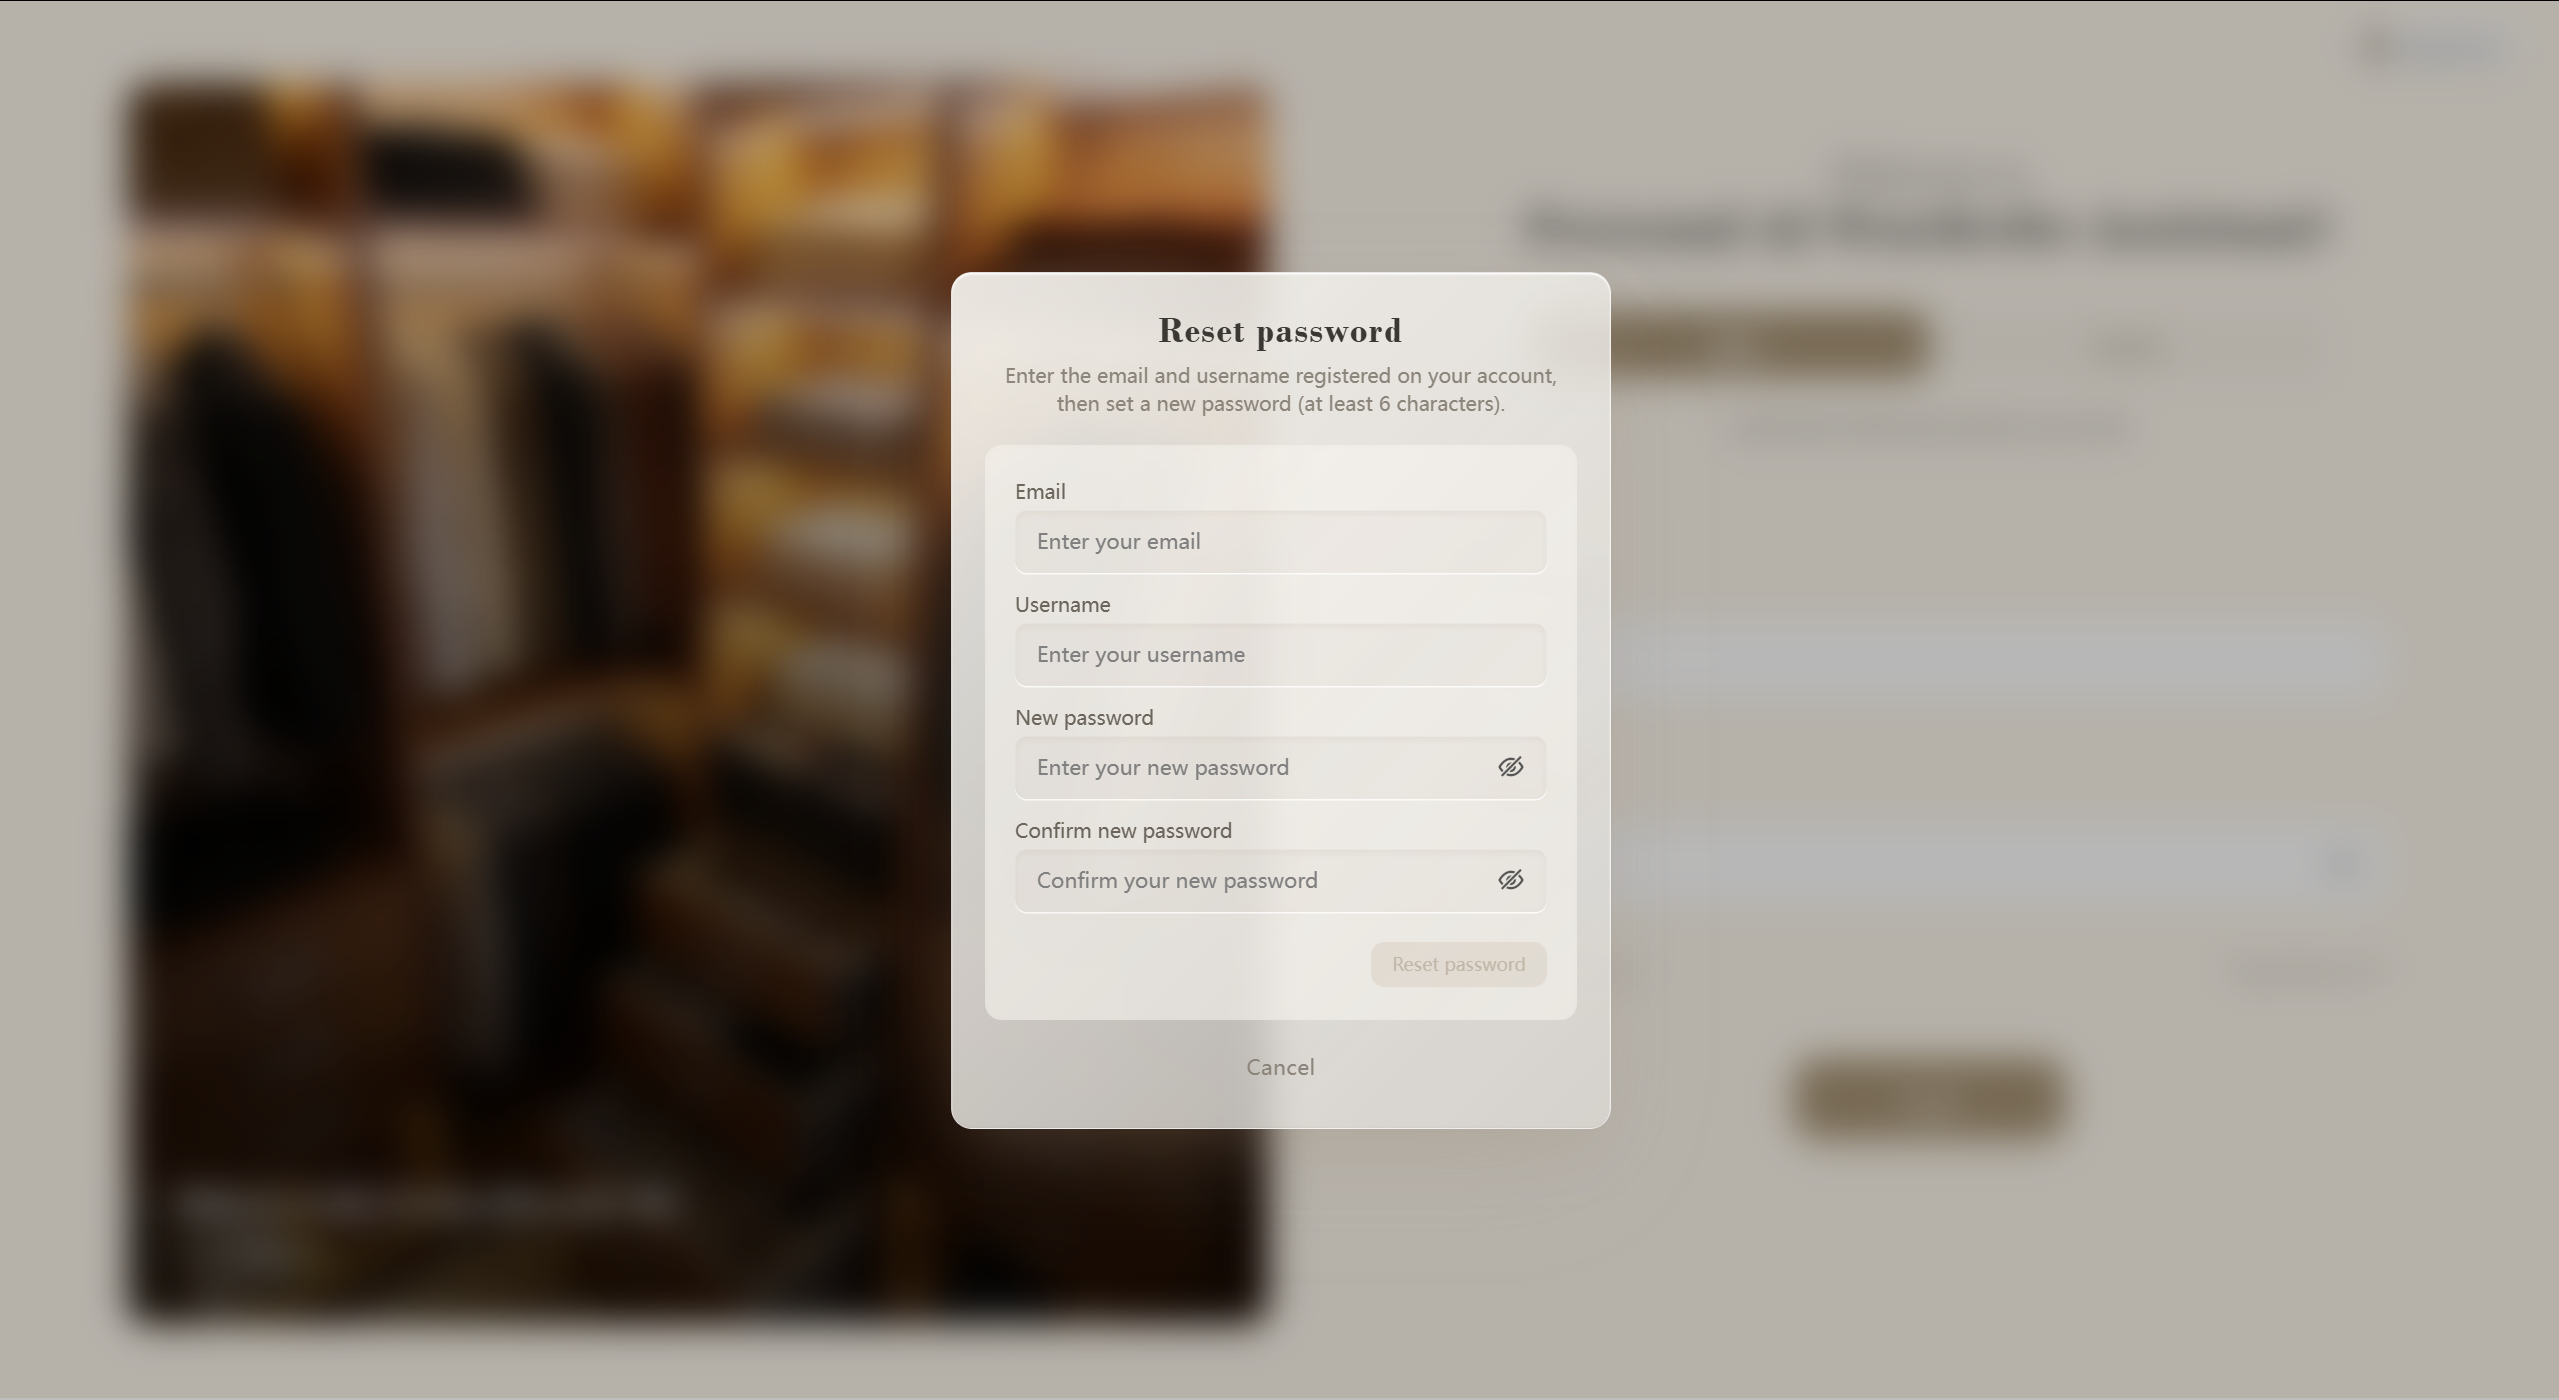
\includegraphics[width=\textwidth]{images/Section_5/newUI/change_password.png}
    \end{minipage}
    \caption{login page (left) and forget-password page (right)}
    \label{fig:ui_login}
\end{figure}


\subsection{Layout structure of main pages}
All pages adopt a two-column layout: the left column lists the main functions, while the right column presents the specific interfaces of each function, as shown in Fig \ref{fig:initial_ui}. This layout separates navigation and content clearly, reducing cognitive load and supporting usability requirement (NFR-05).

\begin{figure}[H]
    \centering
    
\includegraphics[width=1.0\textwidth]{images/Section_5/newUI/initial.png}
    \caption{Initial page}
    \label{fig:initial_ui}
\end{figure}

Below is an introduction to the UI of five main modules of this software:

\textbf{\large a. LLM Recommendation}
\begin{figure}[H]
    \centering
    
\includegraphics[width=1.0\textwidth]{images/Section_5/newUI/LLM.png}
    \caption{LLM Recommendation page}
    \label{fig:llm_ui}
\end{figure}

This page follows the existing navigation design, with a sidebar on the left that displays the user’s query history in chronological order. On the right, users can input their outfit requirements (FR-05), and the system will incorporate weather information (FR-06) to generate recommendations. The generated results are presented in a card-based format with clear explanations (FR-08), making them easy to read and compare. This card-based design improves readability and consistency across outputs, thereby supporting NF-04 and NF-05.

\begin{figure}[H]
    \centering
    % 左图
    \begin{minipage}[b]{0.48\textwidth}
        \centering
        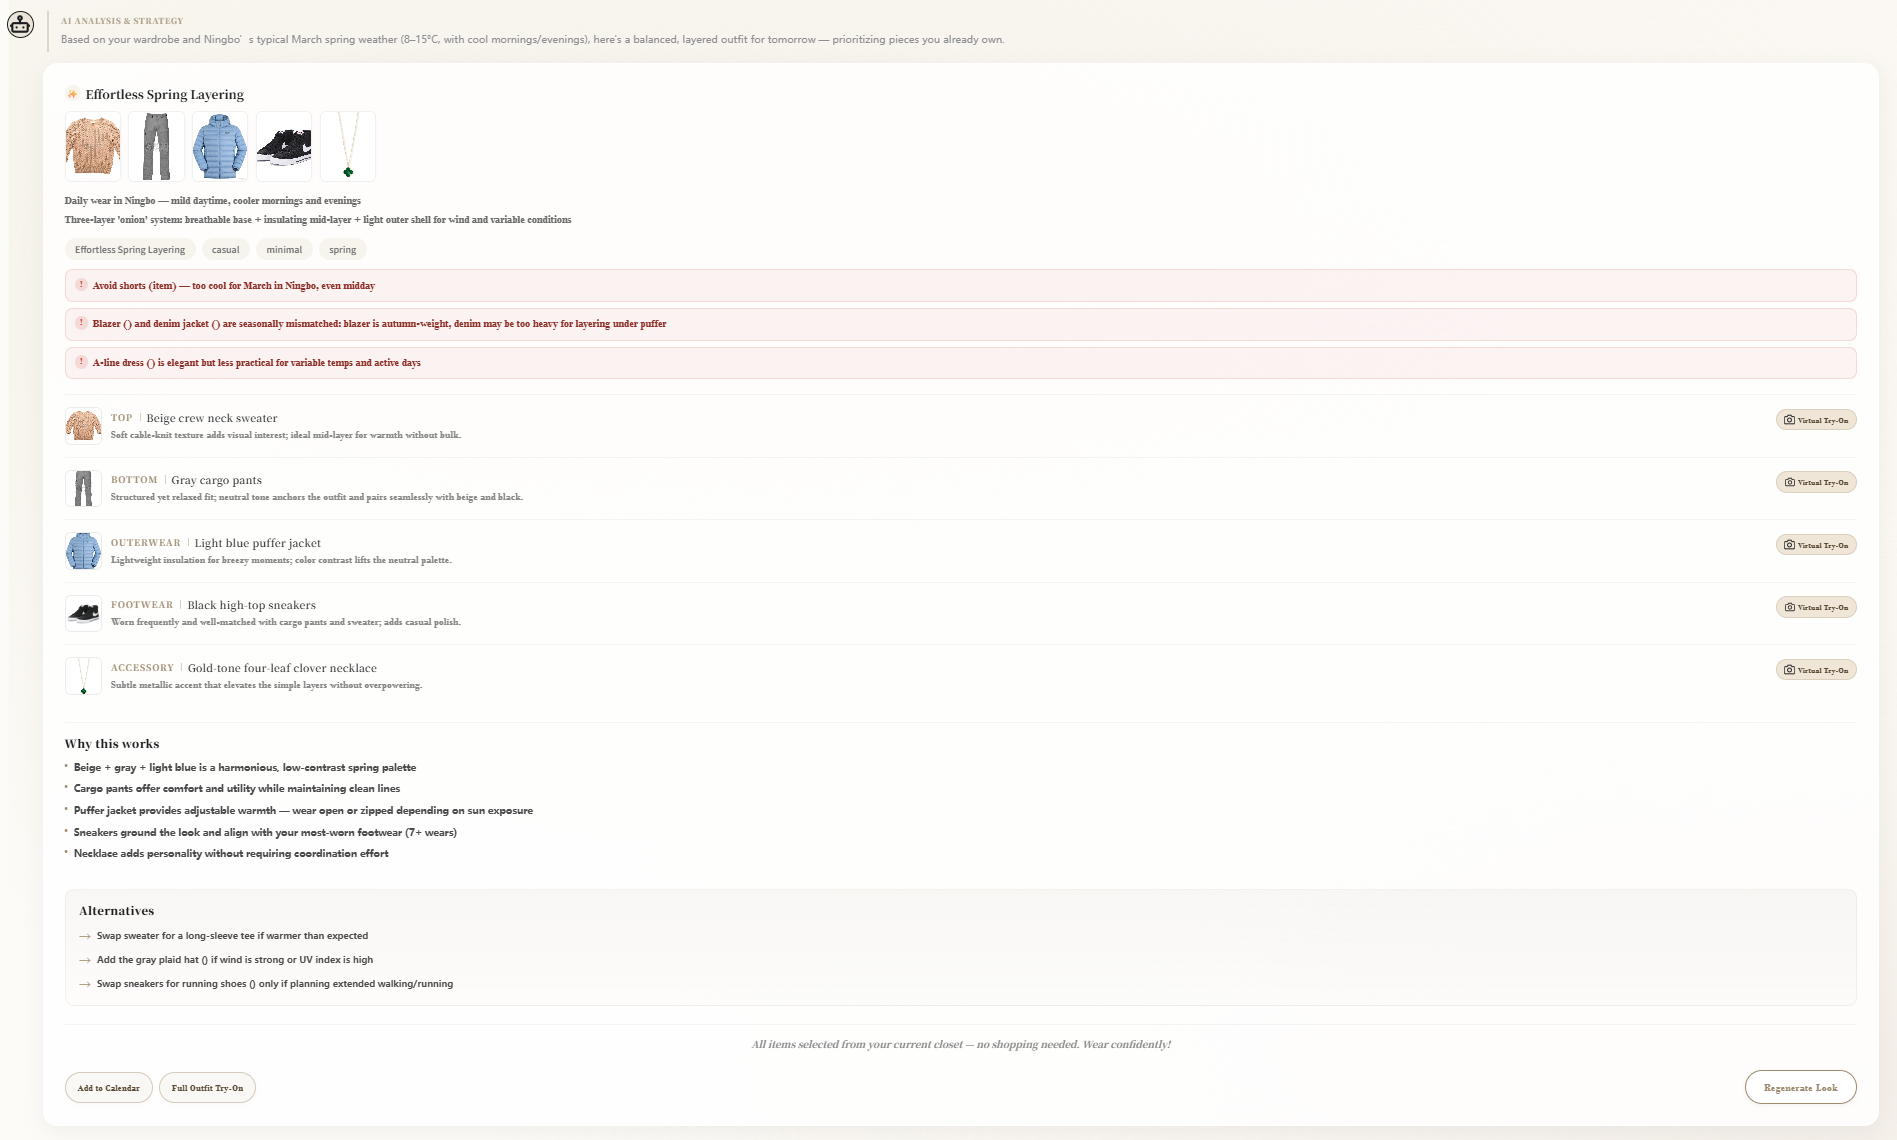
\includegraphics[width=\textwidth]{images/Section_5/newUI/LLM_recommendation.png}
    \end{minipage}
    \hfill
    % 右图
    \begin{minipage}[b]{0.48\textwidth}
        \centering
        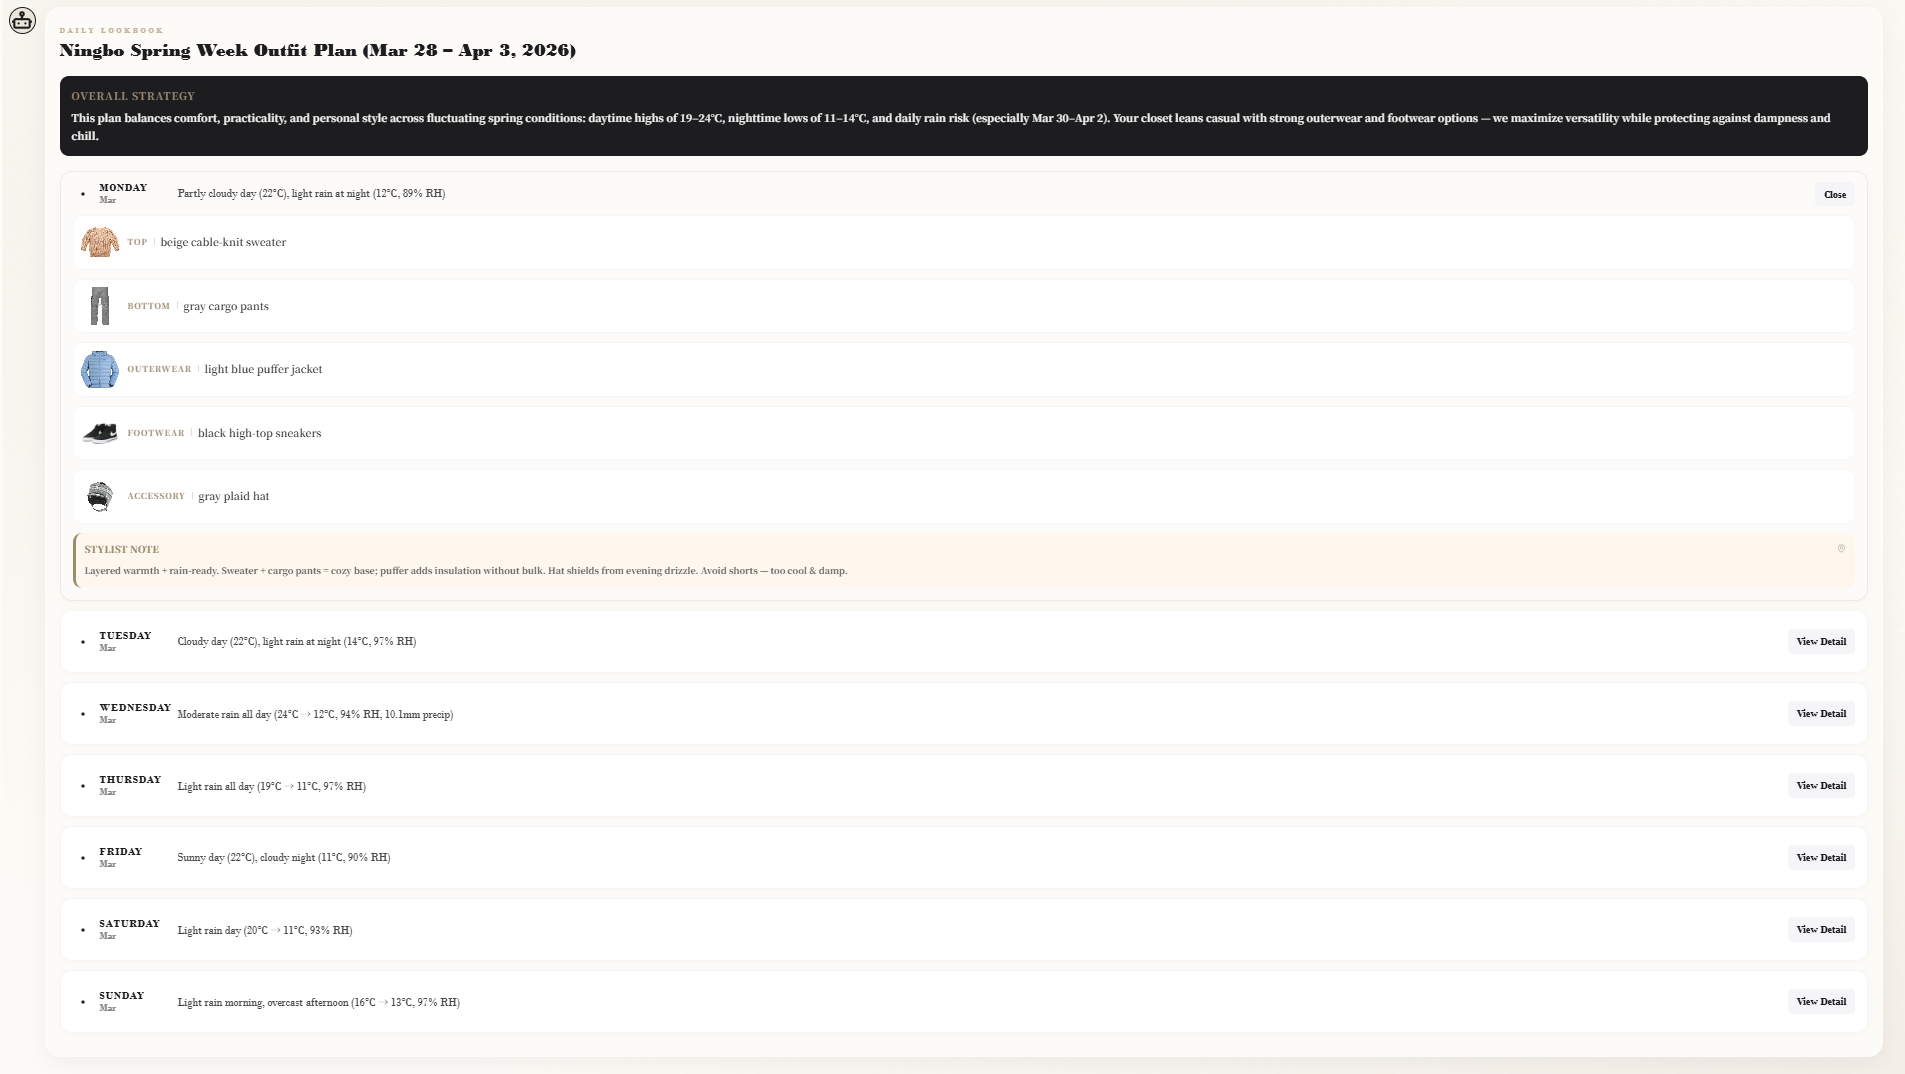
\includegraphics[width=\textwidth]{images/Section_5/newUI/LLM_plan.png}
    \end{minipage}
    \caption{Recommendation format (left) and plan format (right)}
    \label{fig:llm_type}
\end{figure}
Fig.\ref{fig:llm_type} shows that the interface also supports different types of outputs depending on user queries. For example, a recommendation request (e.g. “What should I wear tomorrow?”) produces outfit suggestions, while planning-related queries (e.g. “Plan my outfits for next week”) generate structured plans.

\begin{figure}[H]
    \centering
    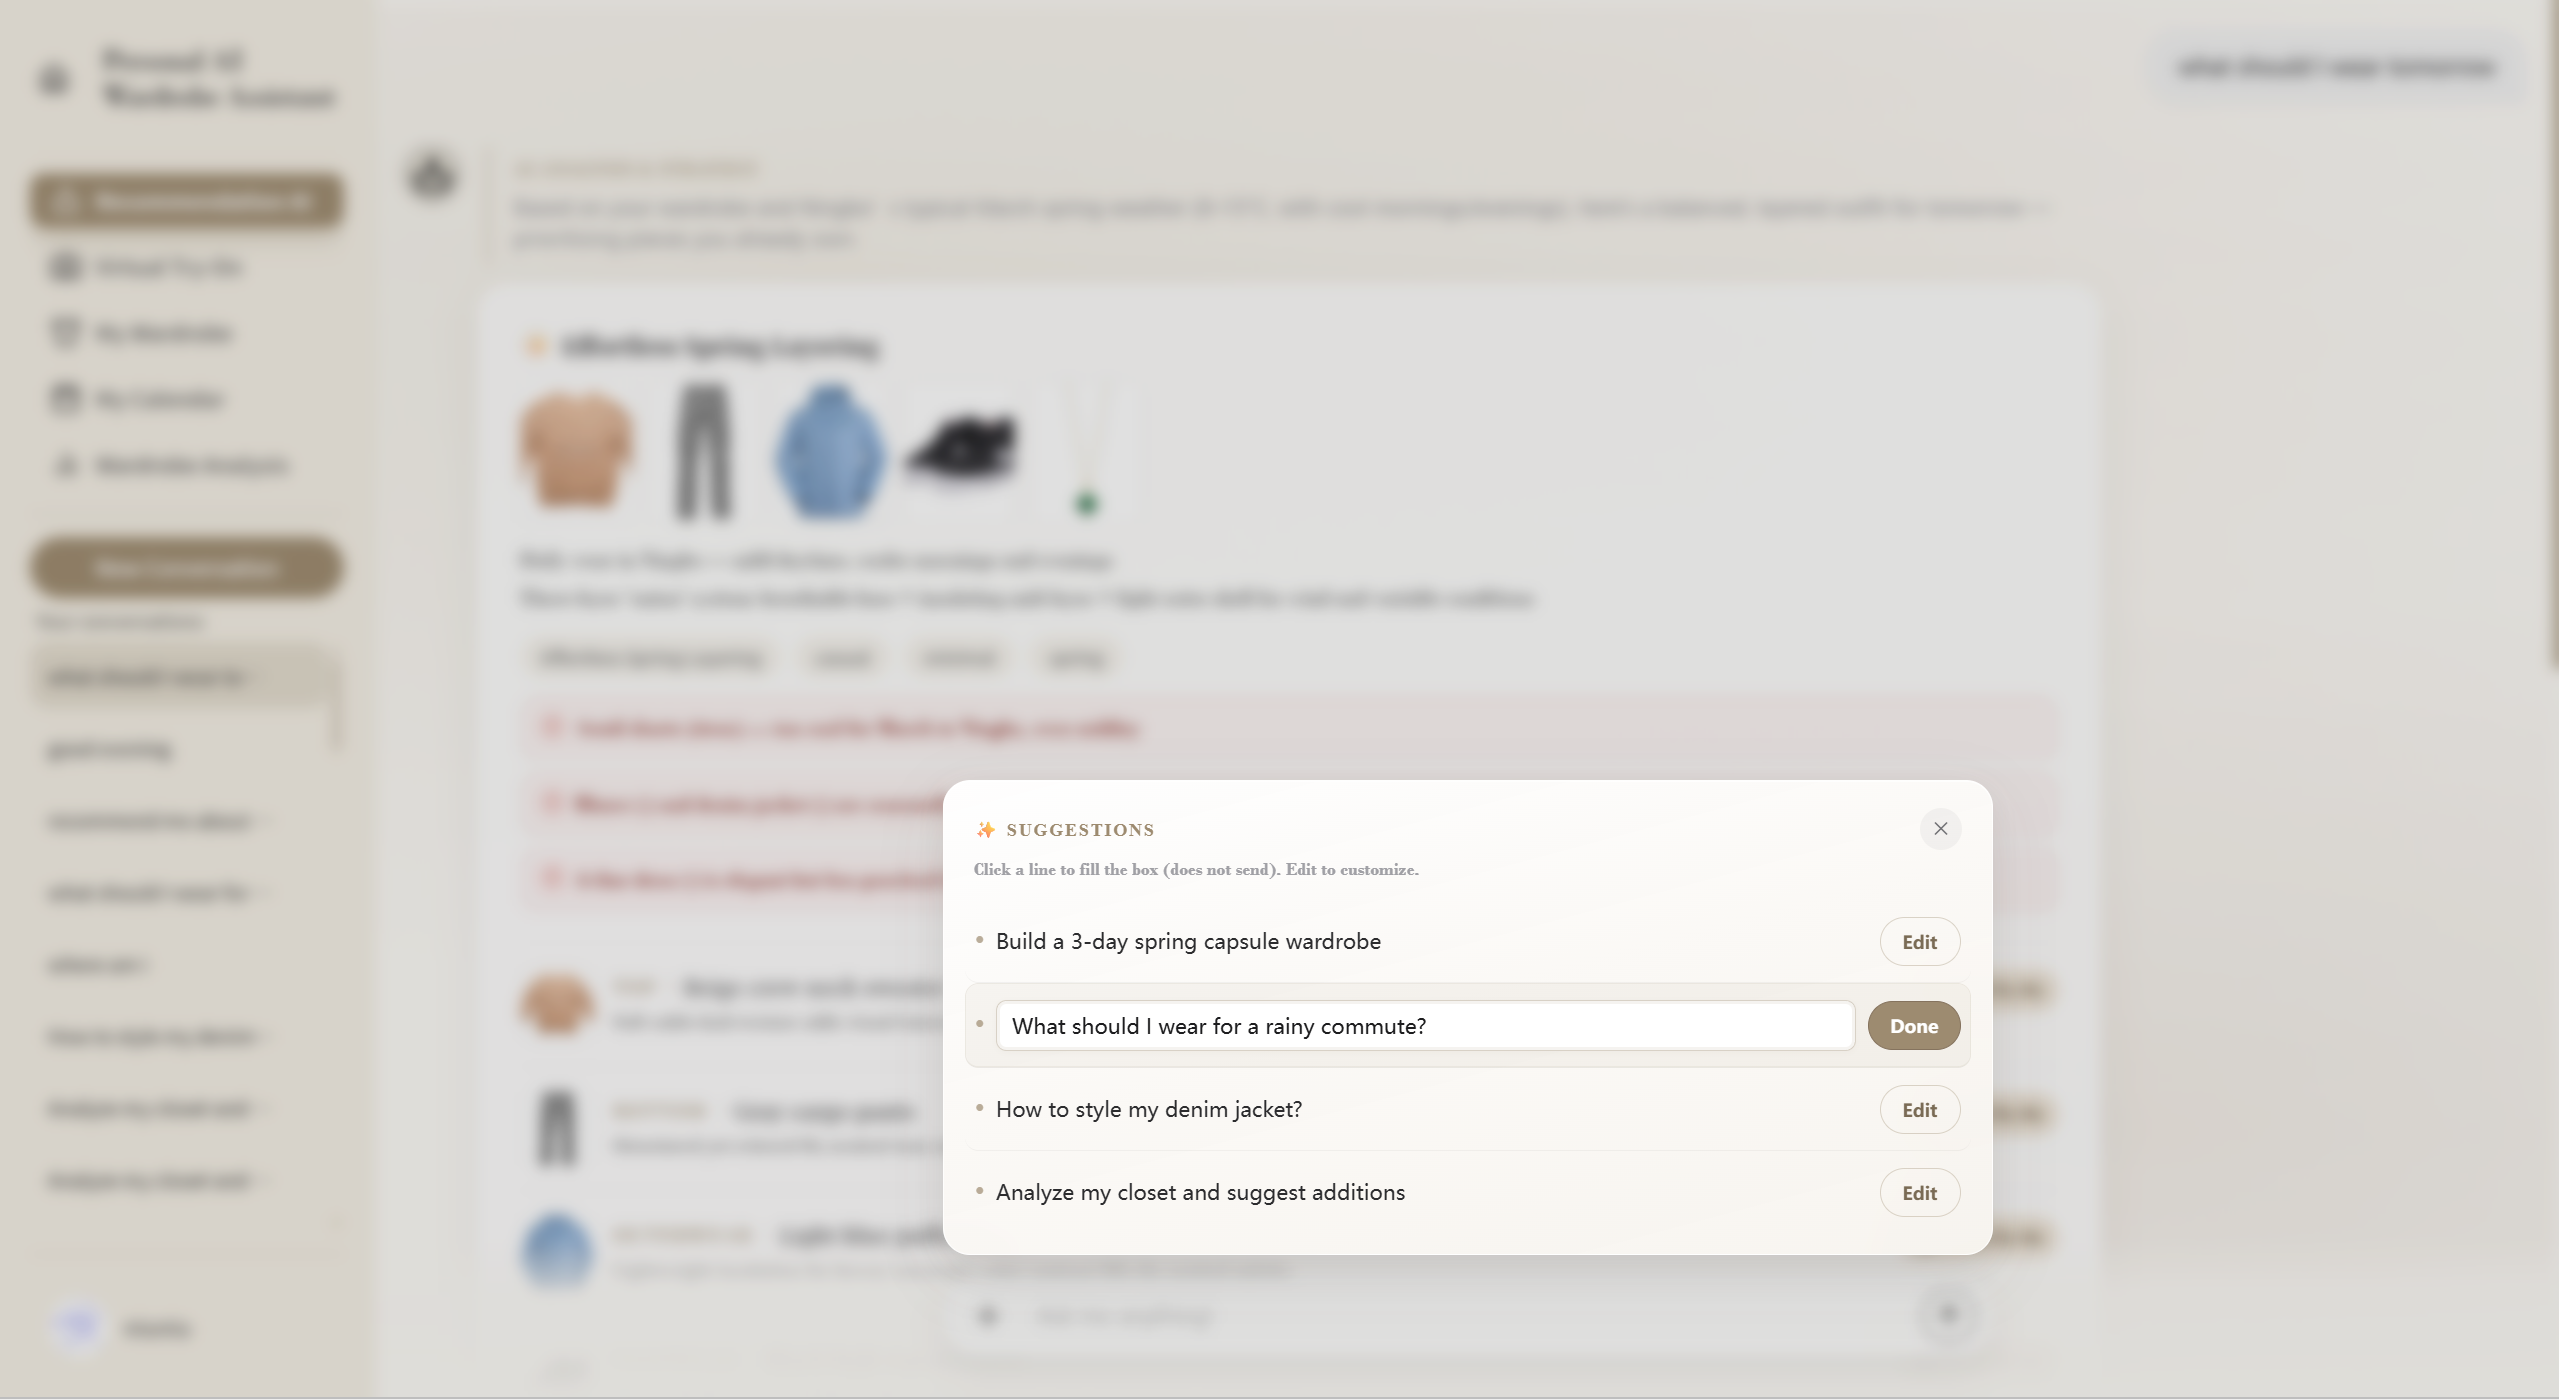
\includegraphics[width=1.0\textwidth]{images/Section_5/newUI/prompt.png}
    \caption{Editable prompts}
    \label{fig:llm_prompt}
\end{figure}

To further improve usability, the interface provides editable shortcut prompts. Users can save and reuse commonly-used queries, which reduces repeated input and improves overall efficiency.\\




\textbf{\large b. Virtual Try-on}
\begin{figure}[H]
    \centering
    
\includegraphics[width=1.0\textwidth]{images/Section_5/newUI/VTO.png}
    \caption{Virtual Try-On page}
    \label{fig:VTO_ui}
\end{figure}
The virtual try-on page mainly consists of two upload panels, used for uploading a full-body photo of the user and an image of the clothing item respectively (FR-10). After the upload is completed, the system will generate and display the try-on result (FR-12).

This simple workflow (upload → generate → preview) reduces user effort and supports the usability requirement (NF-05).\\



\textbf{\large c. Wardrobe Management}

\begin{figure}[H]
    \centering
    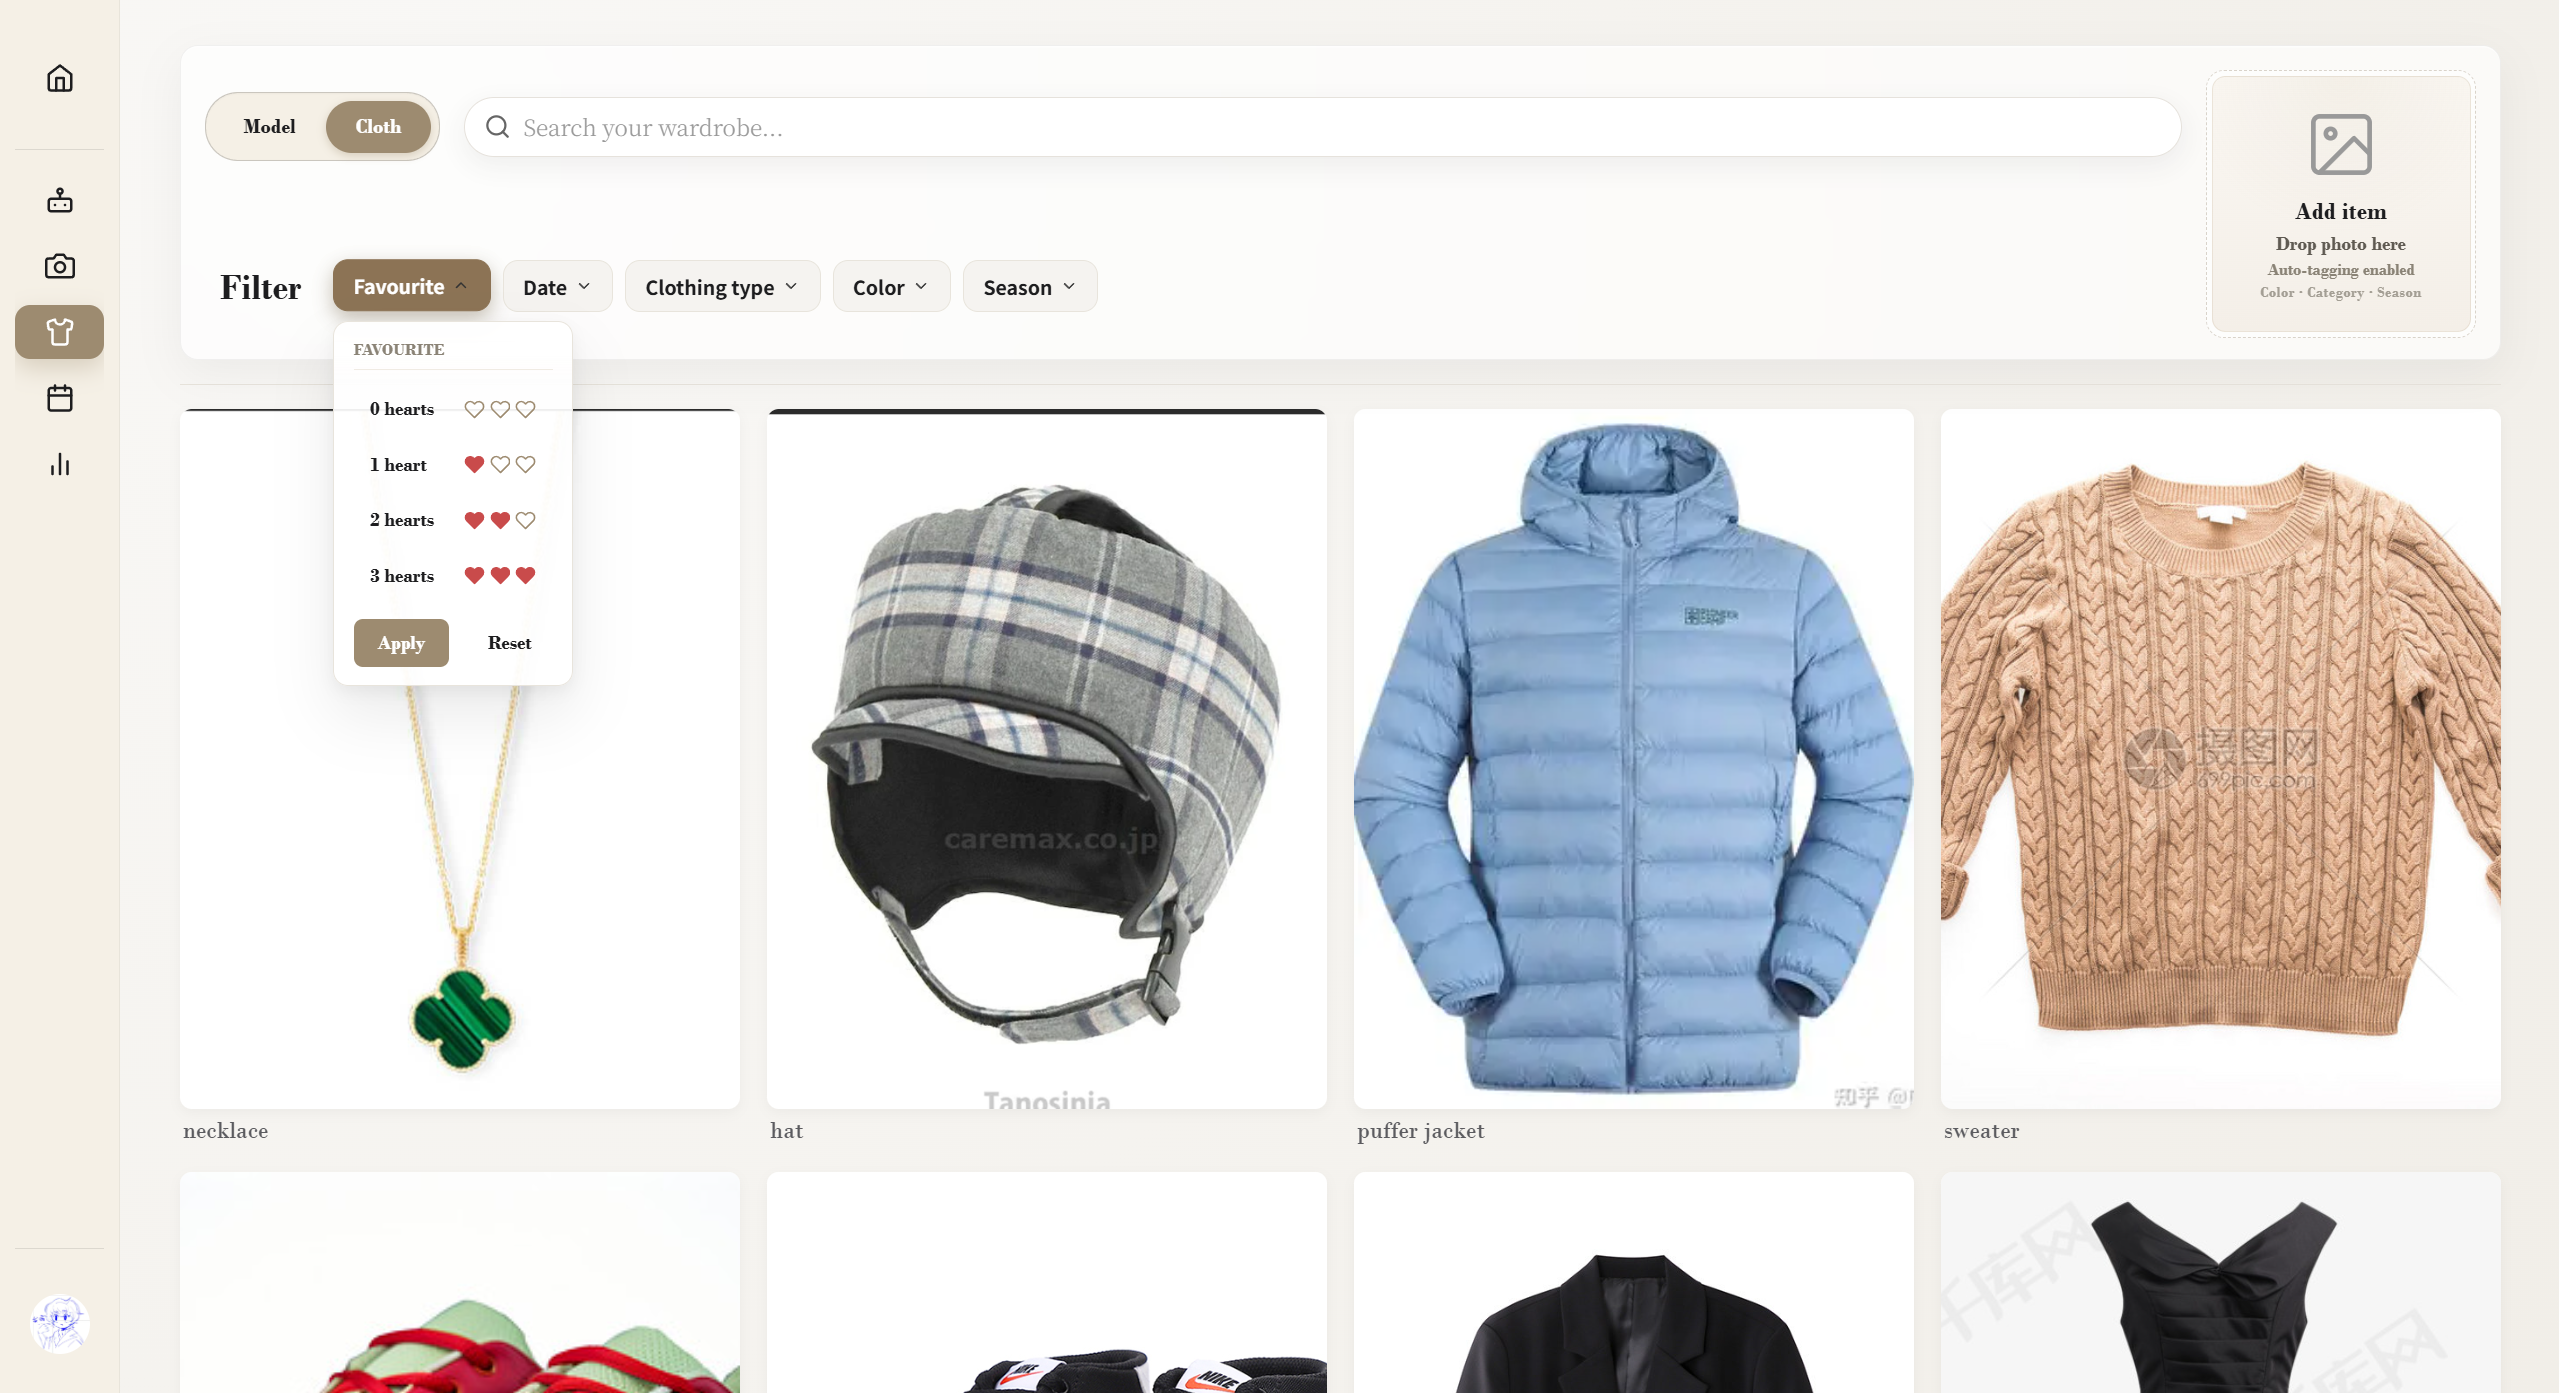
\includegraphics[width=0.8\textwidth]{images/Section_5/newUI/management_mian.png}
    \caption{Wardrobe Management page}
    \label{fig:management_ui}
\end{figure}

This page allows users to manage their clothing items through a clear and structured interface. Users can add new items using the upload panel at the top (FR-02), while a search bar and multiple filter options can help them find specific clothes more easily (FR-13). Meanwhile, clothing items are displayed in a grid layout, making it easy for users to browse their wardrobe. 

\begin{figure}[H]
    \centering
    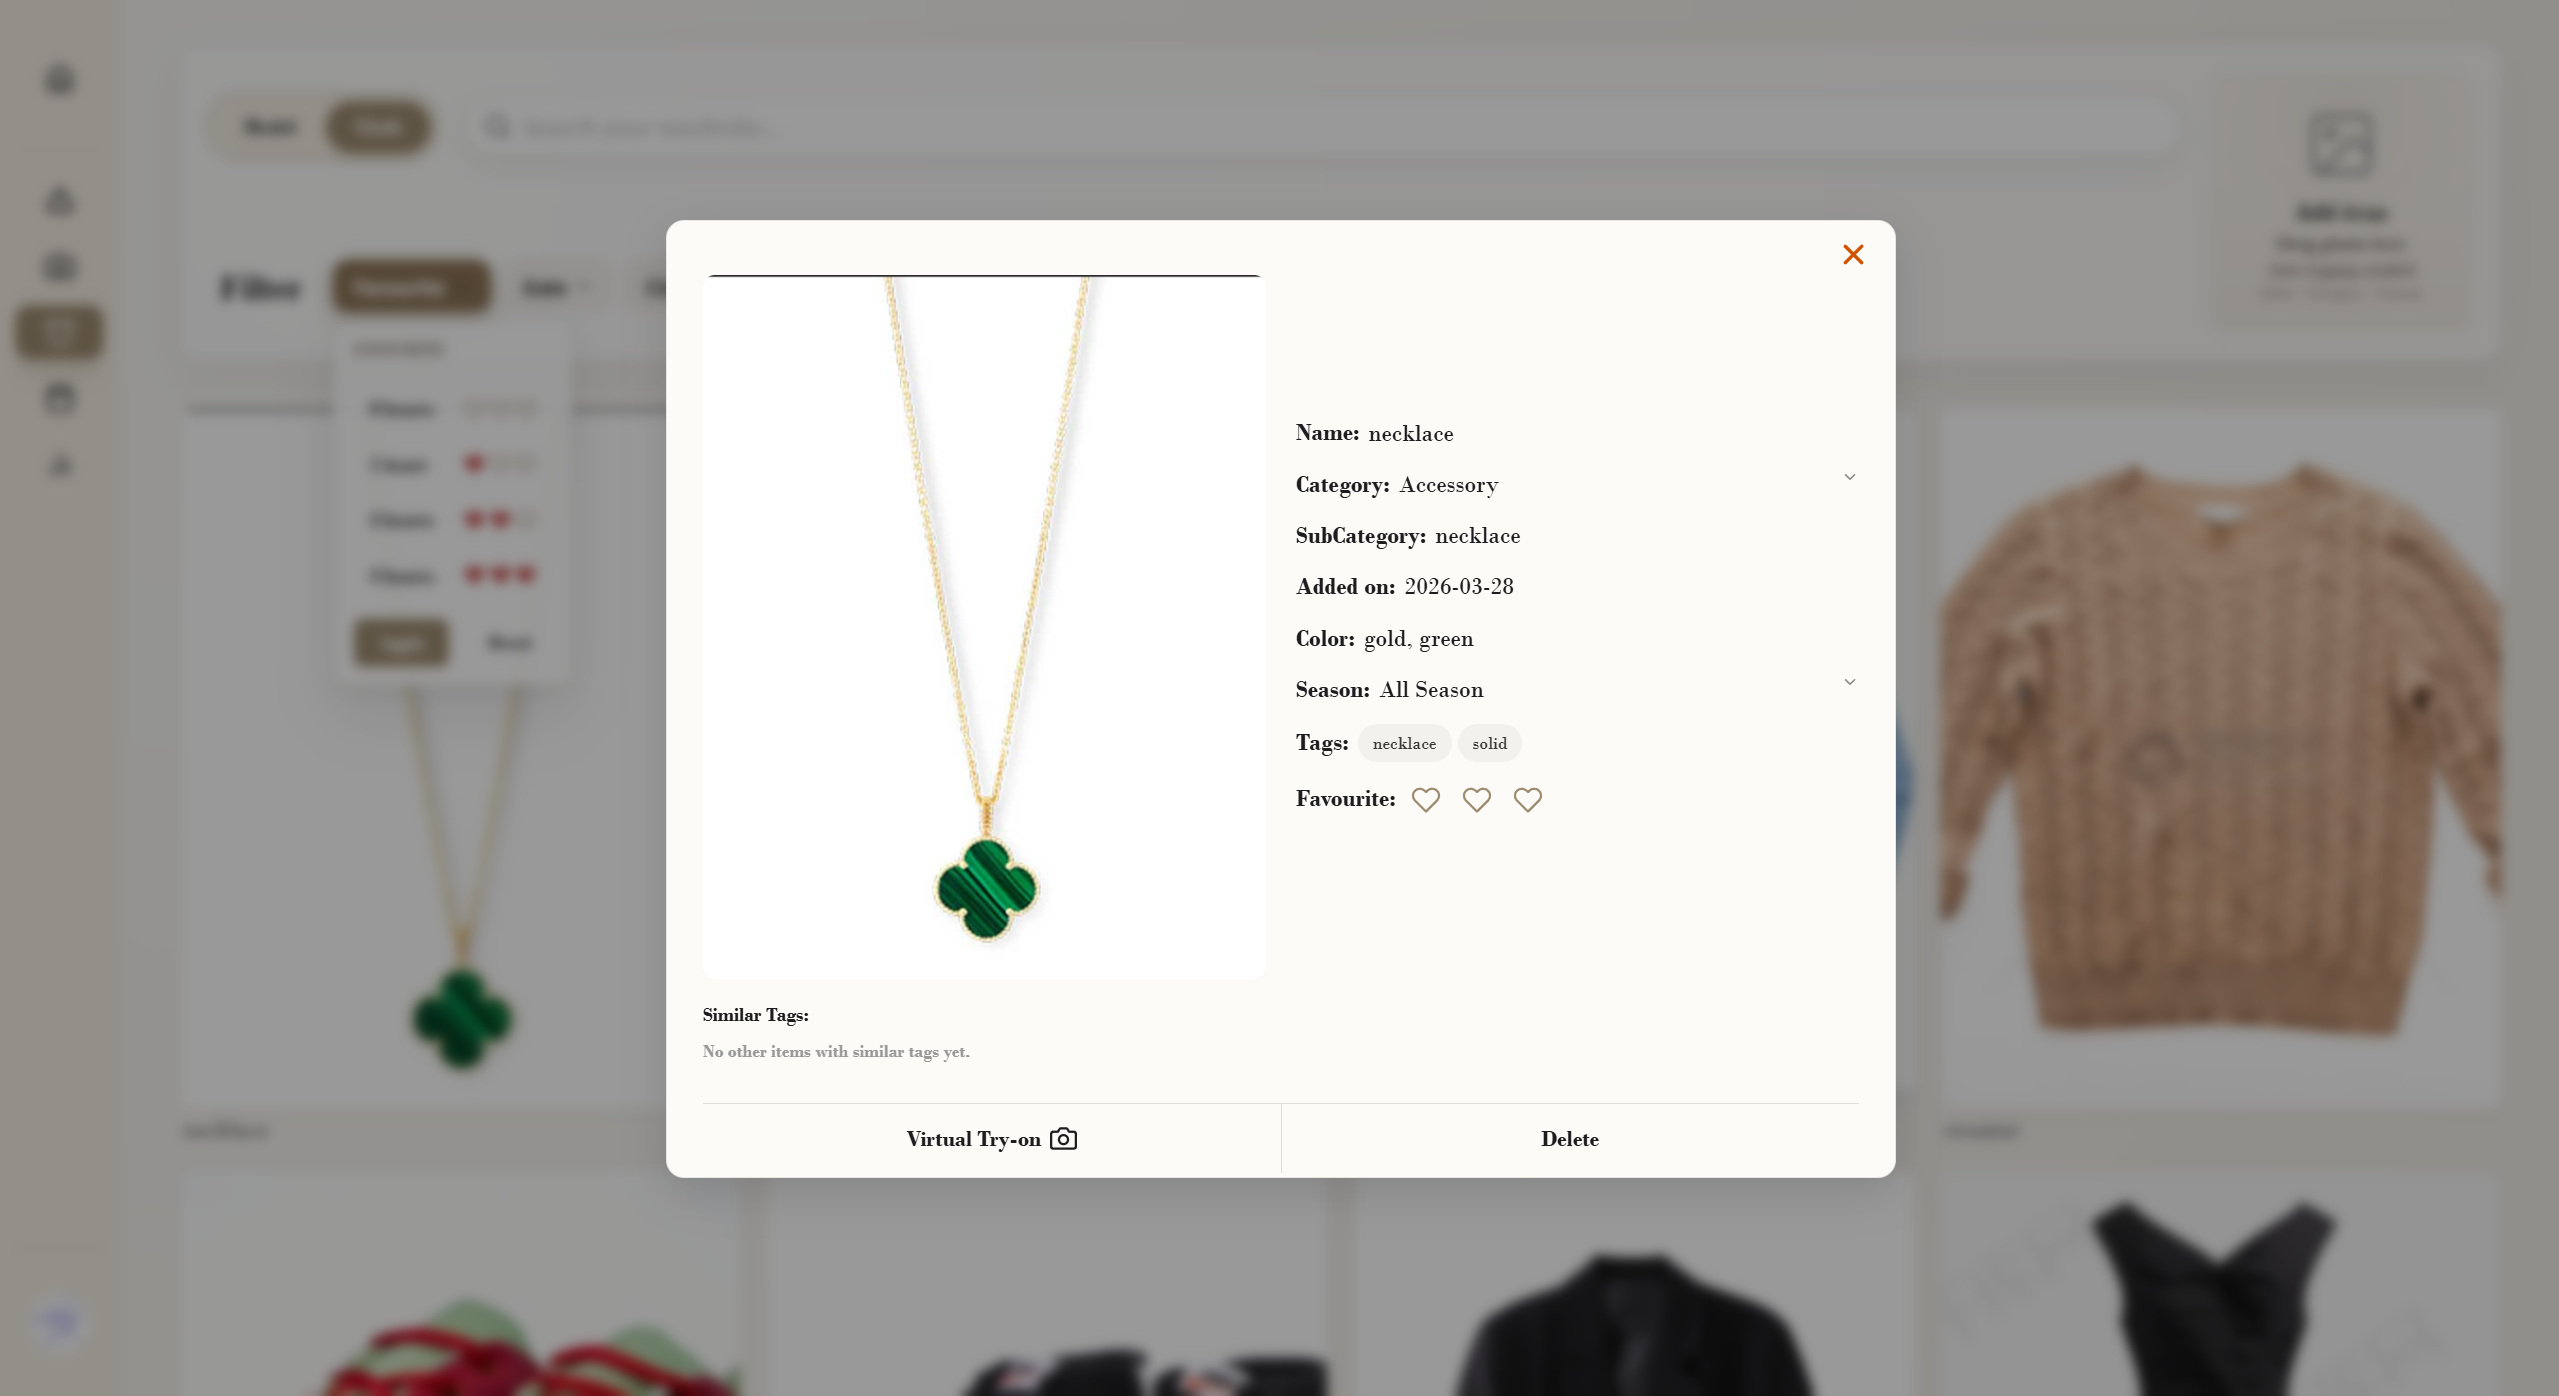
\includegraphics[width=0.7\textwidth]{images/Section_5/newUI/management_detail.png}
    \hfill
    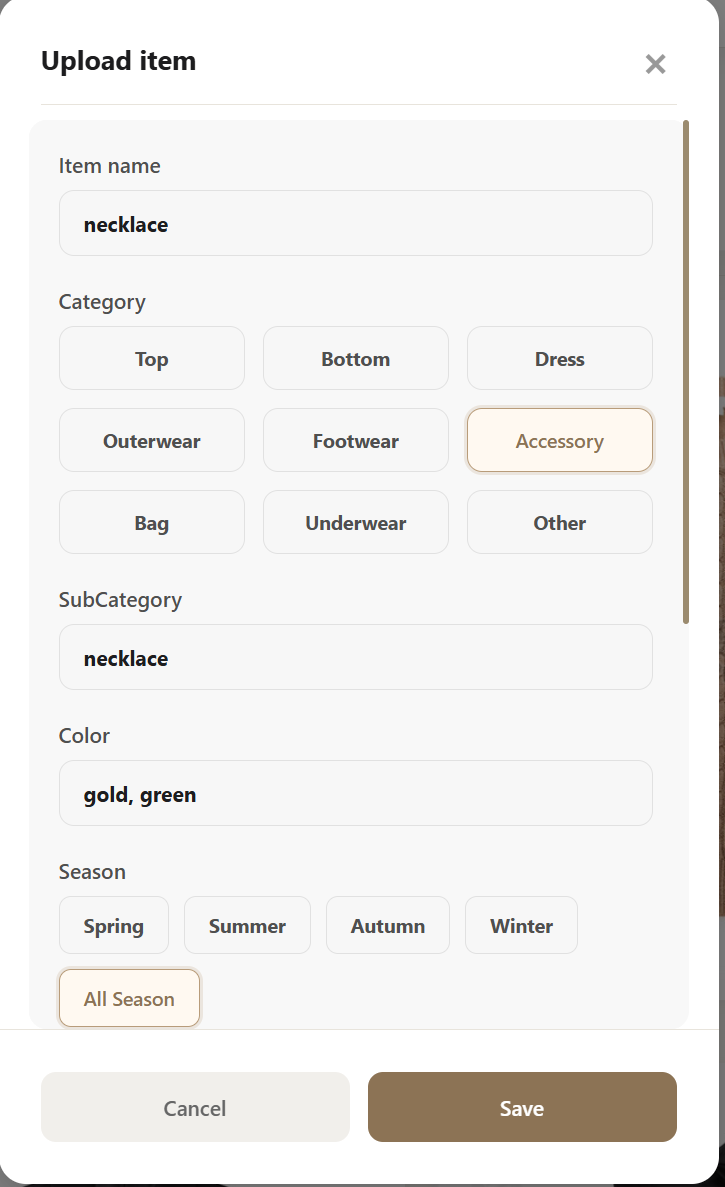
\includegraphics[width=0.25\textwidth]{images/Section_5/newUI/management_upload.png}
    \caption{Clothing detail view (left) and upload dialog (right)}
    \label{fig:wardrobe_detail_upload}
\end{figure}

Users can click on each item card to view more detailed information. When new items are uploaded, the system automatically generates tags instead of requiring manual input, which reduces user effort and makes the process more smooth.

Overall, this page is designed to keep the interaction simple, allowing users to manage their wardrobe with only a small number of steps. \\



\textbf{\large d. My Calendar}
\begin{figure}[H]
    \centering
    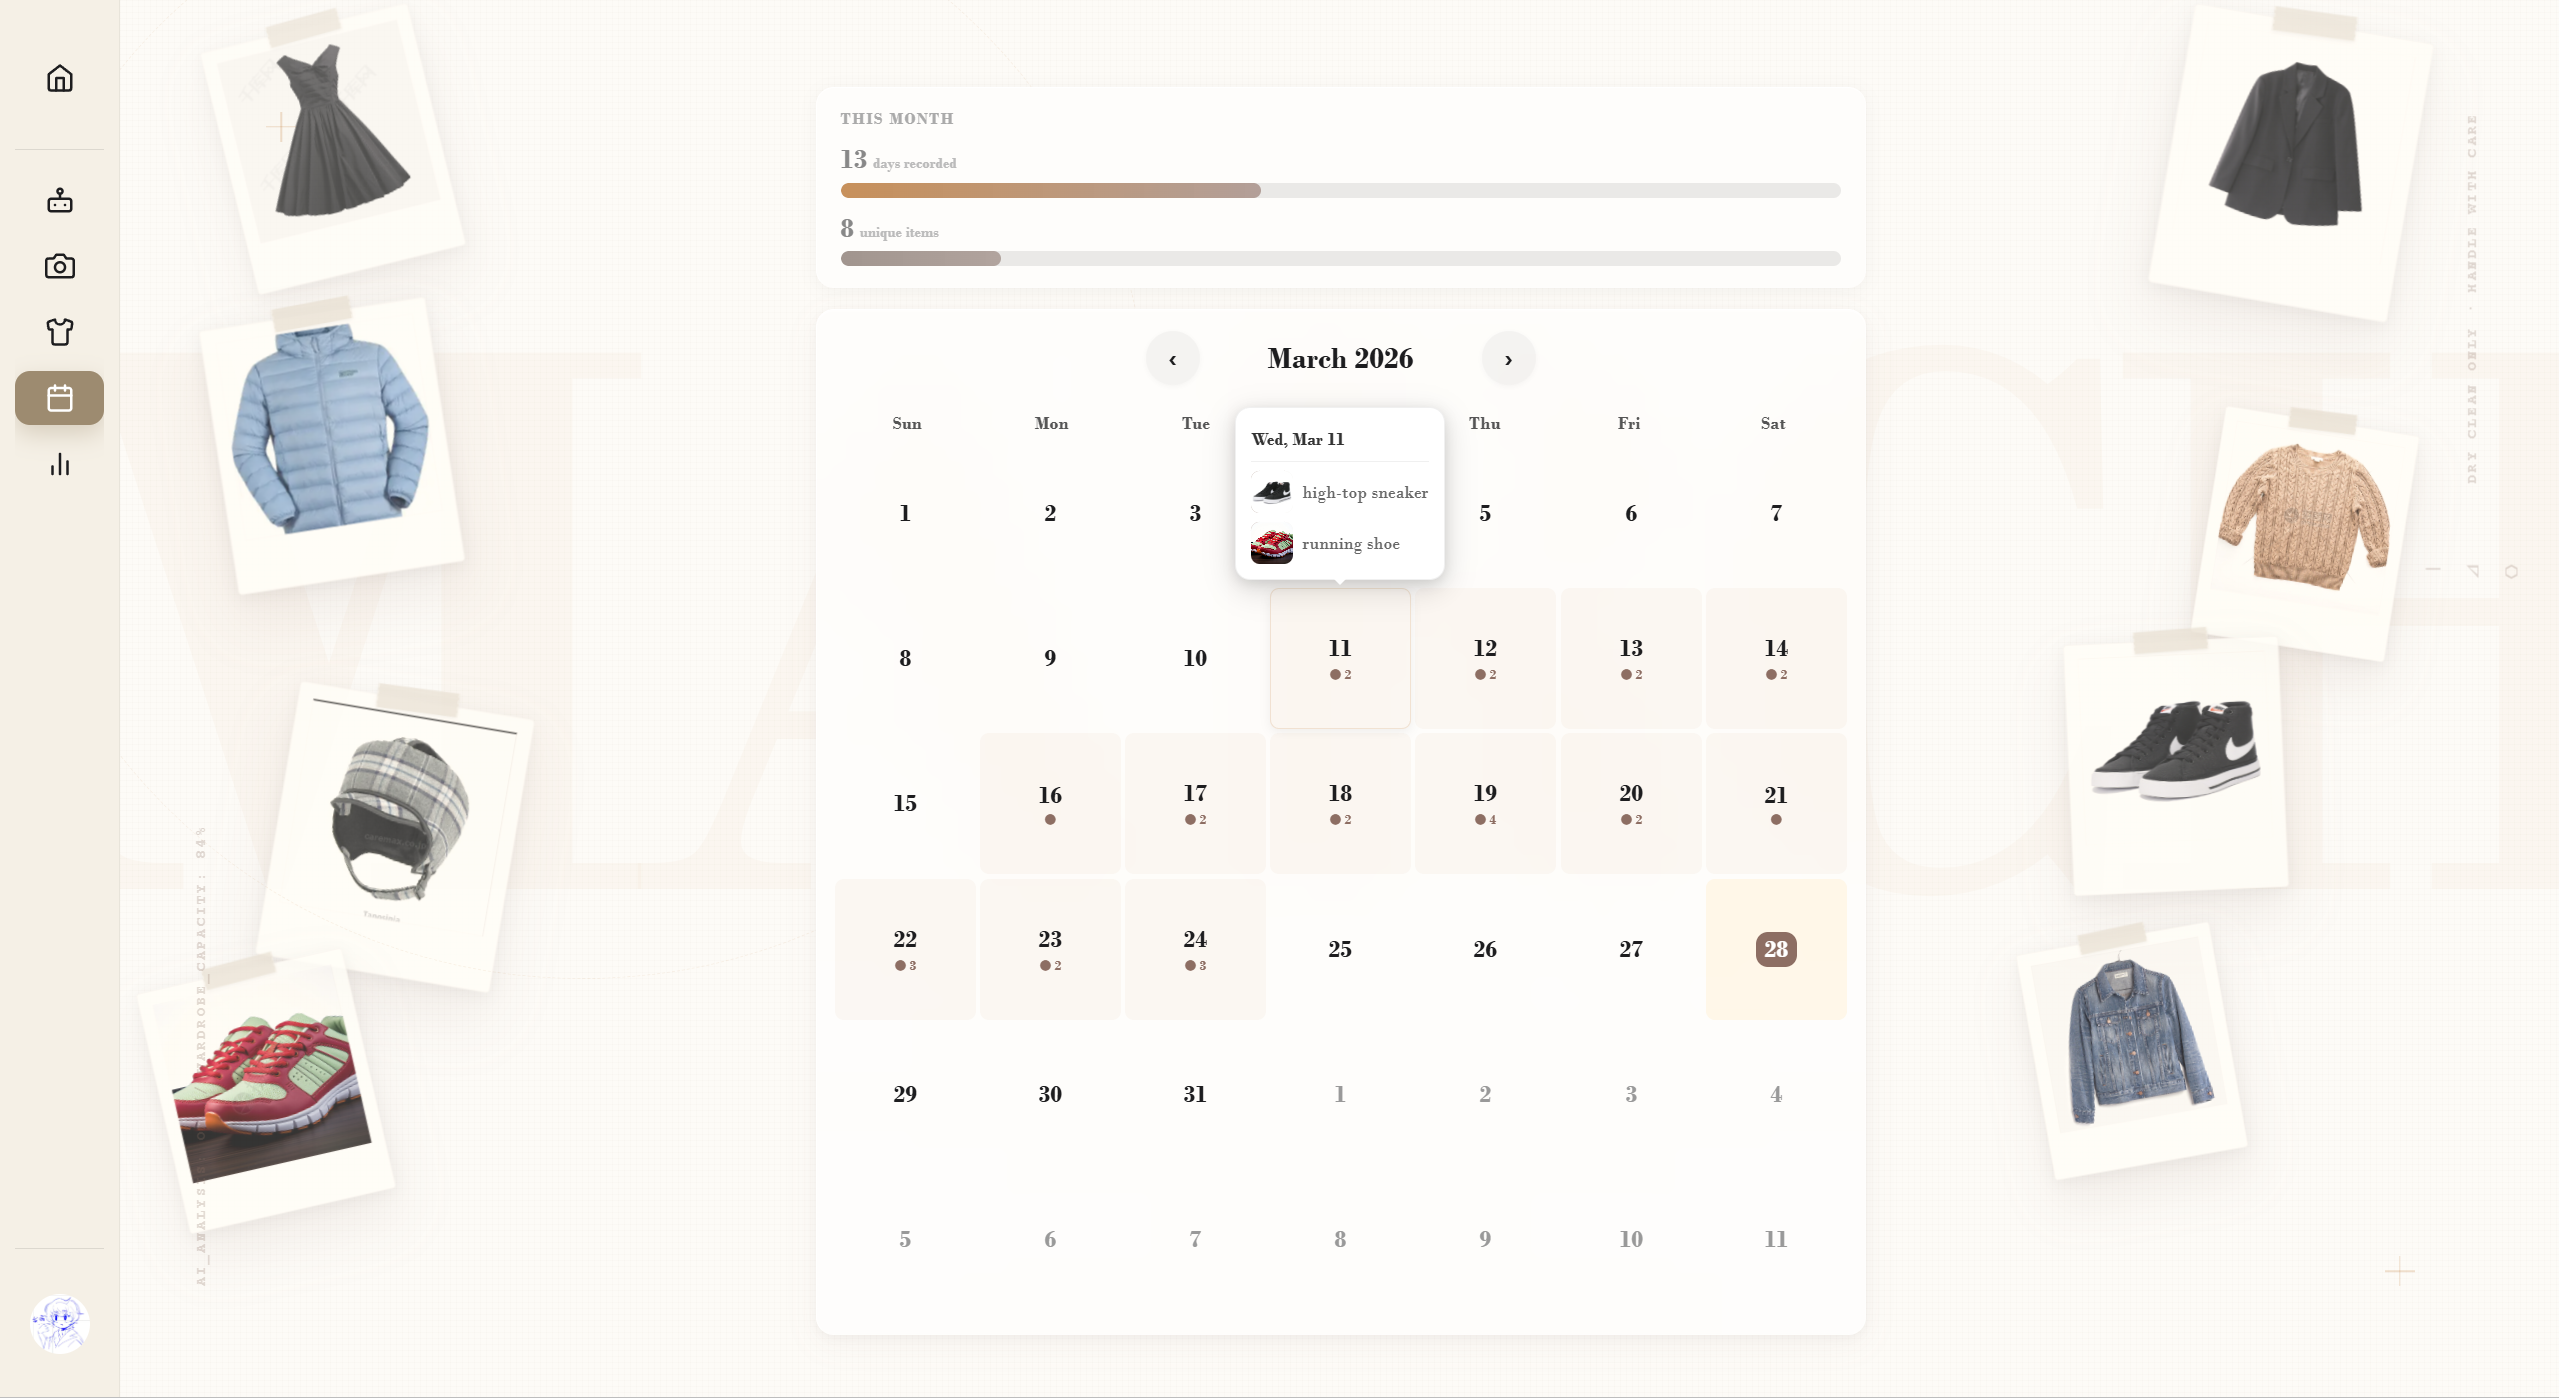
\includegraphics[width=0.8\textwidth]{images/Section_5/newUI/calendar1.png}
    \\[0.5cm]
    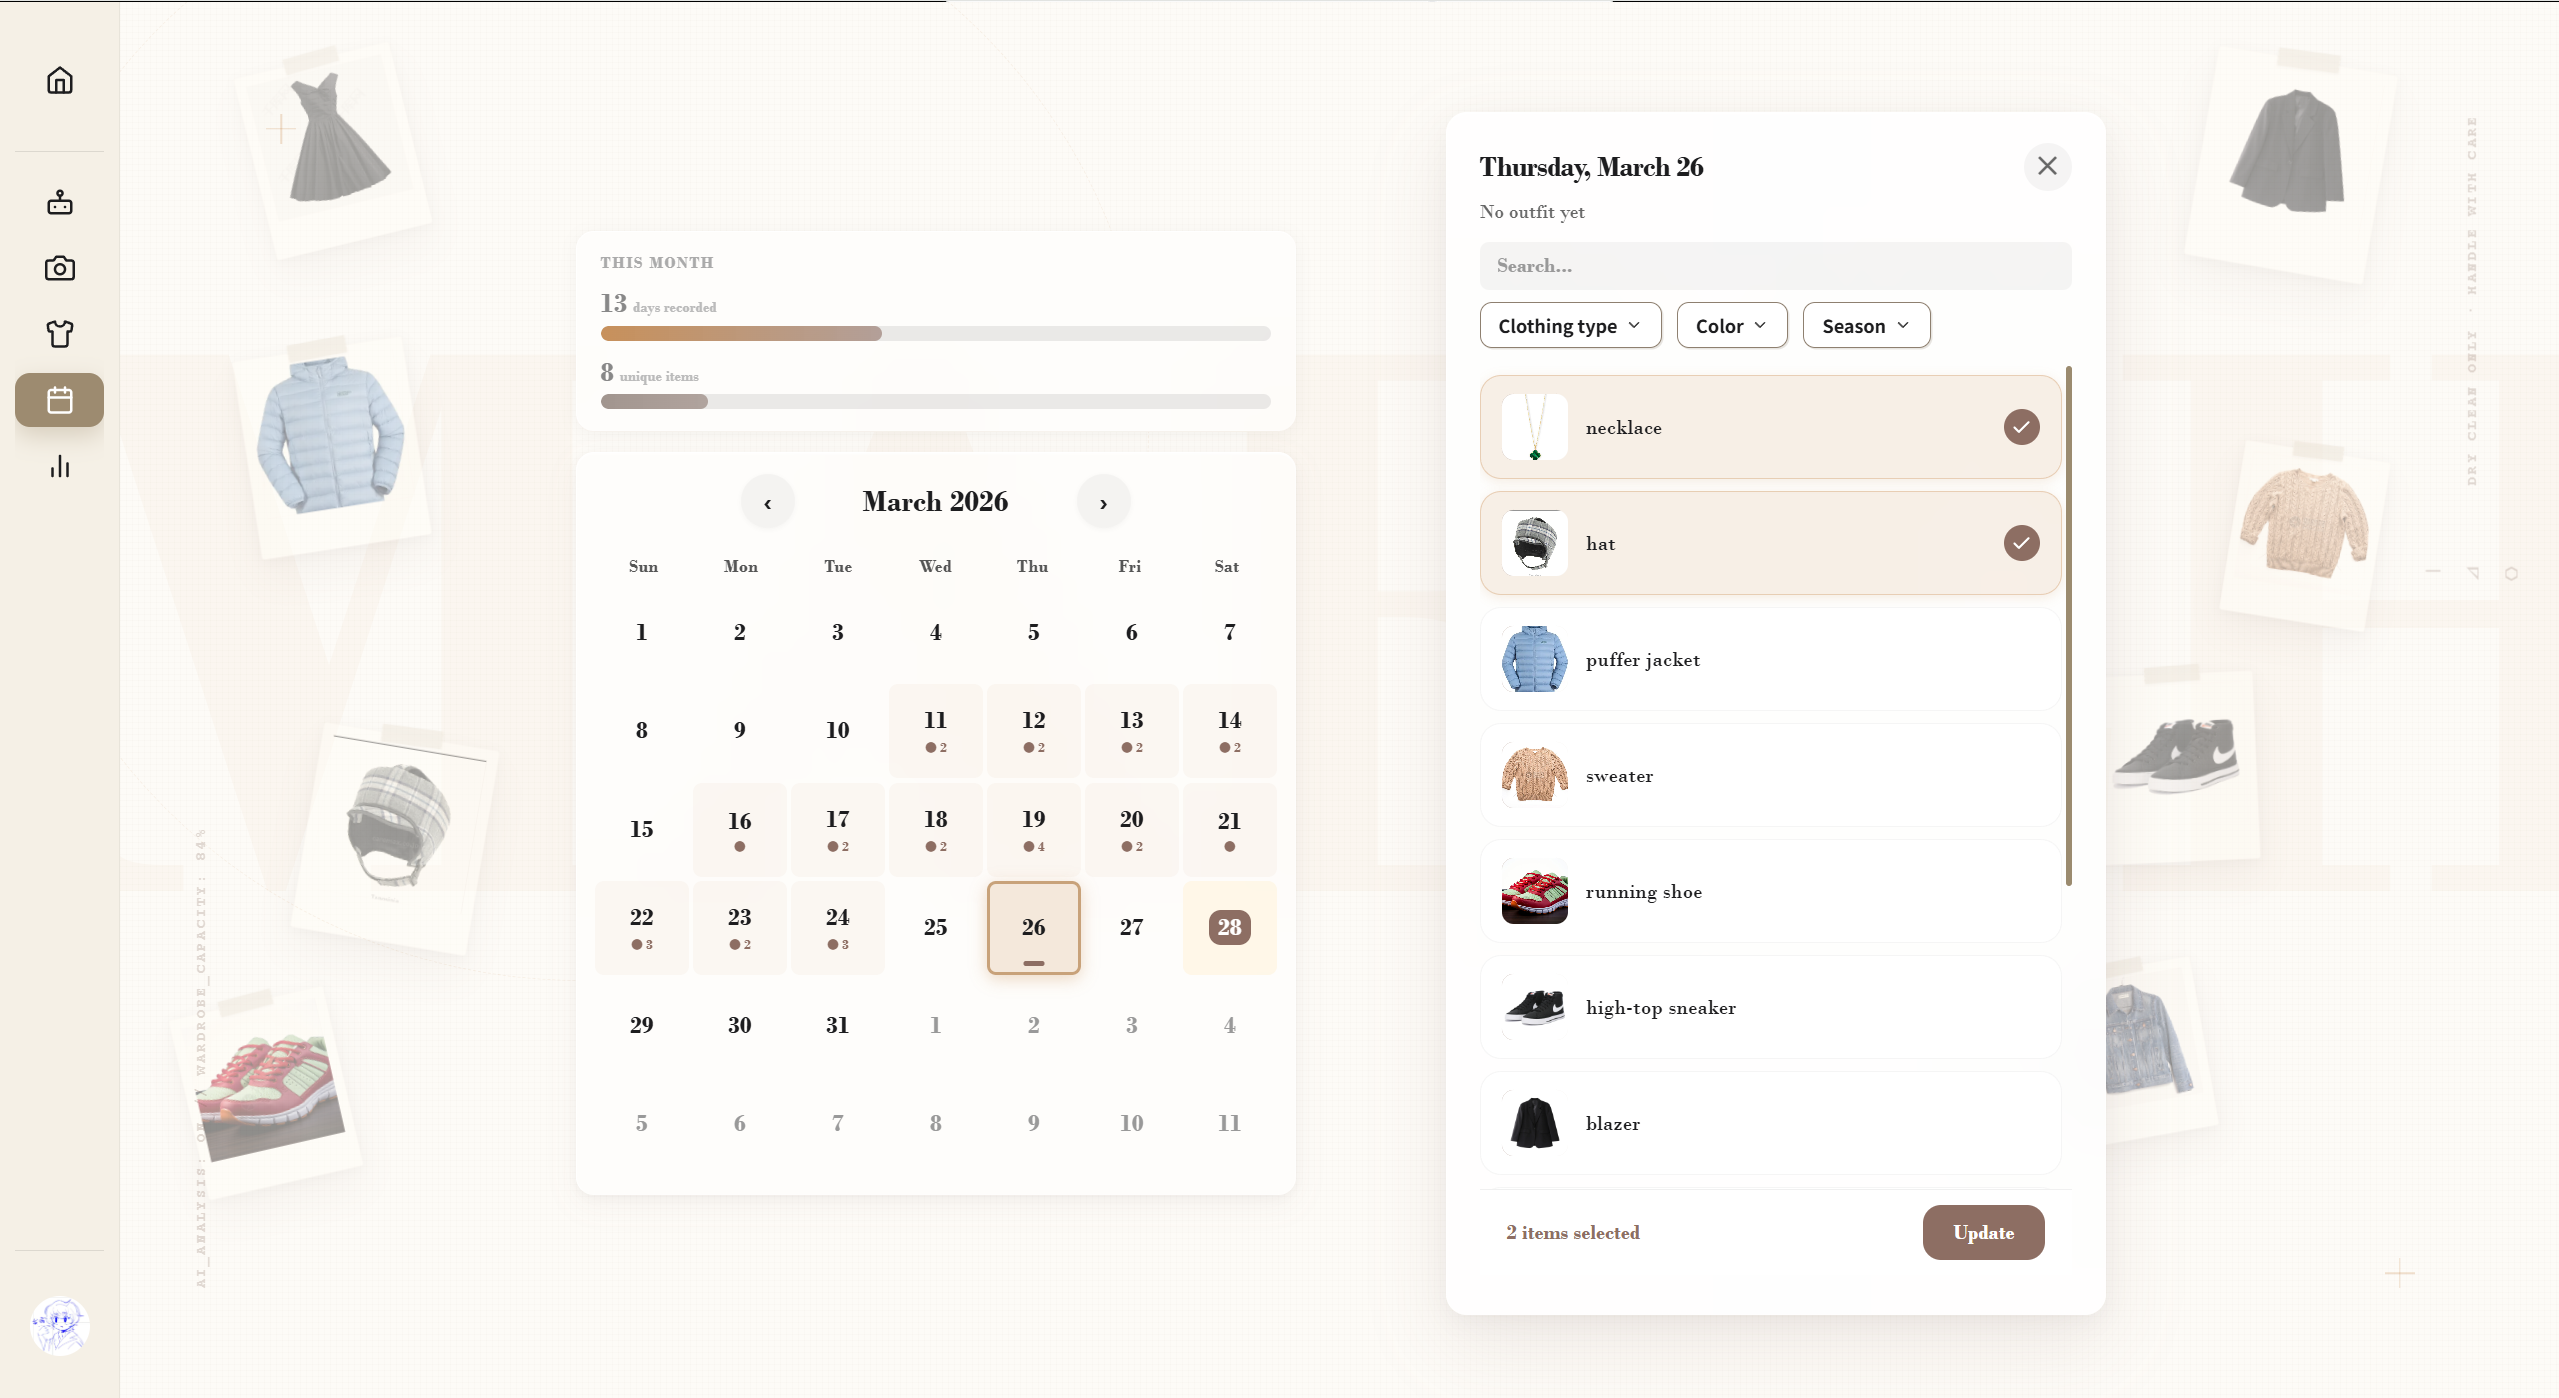
\includegraphics[width=0.8\textwidth]{images/Section_5/newUI/calendar2.png}
    \caption{Calendar (top) and side panel (bottom)}
    \label{fig:VTO_combined}
\end{figure}
This page presents daily outfit records using a calendar layout, where each date shows the outfits worn. Users can either add items manually from their wardrobe or import recommendations from the AI module, supporting smooth interaction between features.

When a date is selected, a side panel helps users choose clothing more easily. The background also includes a polaroid-style photo wall that randomly displays outfits from the current month, making the page more engaging while keeping the interaction simple. This design enhances user engagement while maintaining simplicity, supporting visual consistency (NFR-04).\\


\textbf{\large e. Wardrobe Analysis}
\begin{figure}[H]
    \centering
    
\includegraphics[width=1.0\textwidth]{images/Section_5/newUI/analysis.png}
    \caption{Wardrobe Analysis page}
    \label{fig:Wardrobe_analysis_ui}
\end{figure}
This page presents the wardrobe data indicators through multiple independent information cards. Each card focuses on a separate wardrobe KPI, such as wear frequency, idle rate, and category distribution, allowing users to quickly understand the overall condition of their wardrobe.

In addition to summary metrics, visual elements such as charts and breakdown diagrams are used to improve readability and make the data easier to interpret. The page also provides suggestions based on the analysis results, helping users identify missing items or improve their wardrobe composition.


\subsection{Design Evolution}

Overall, the final UI design remains largely consistent with the initial Figma prototype. However, several design adjustments were made during development after identifying usability issues. These changes mainly focus on improving readability, layout efficiency, and user interaction.

\textbf{(1) Recommendation AI module}

\begin{figure}[H]
    \centering
    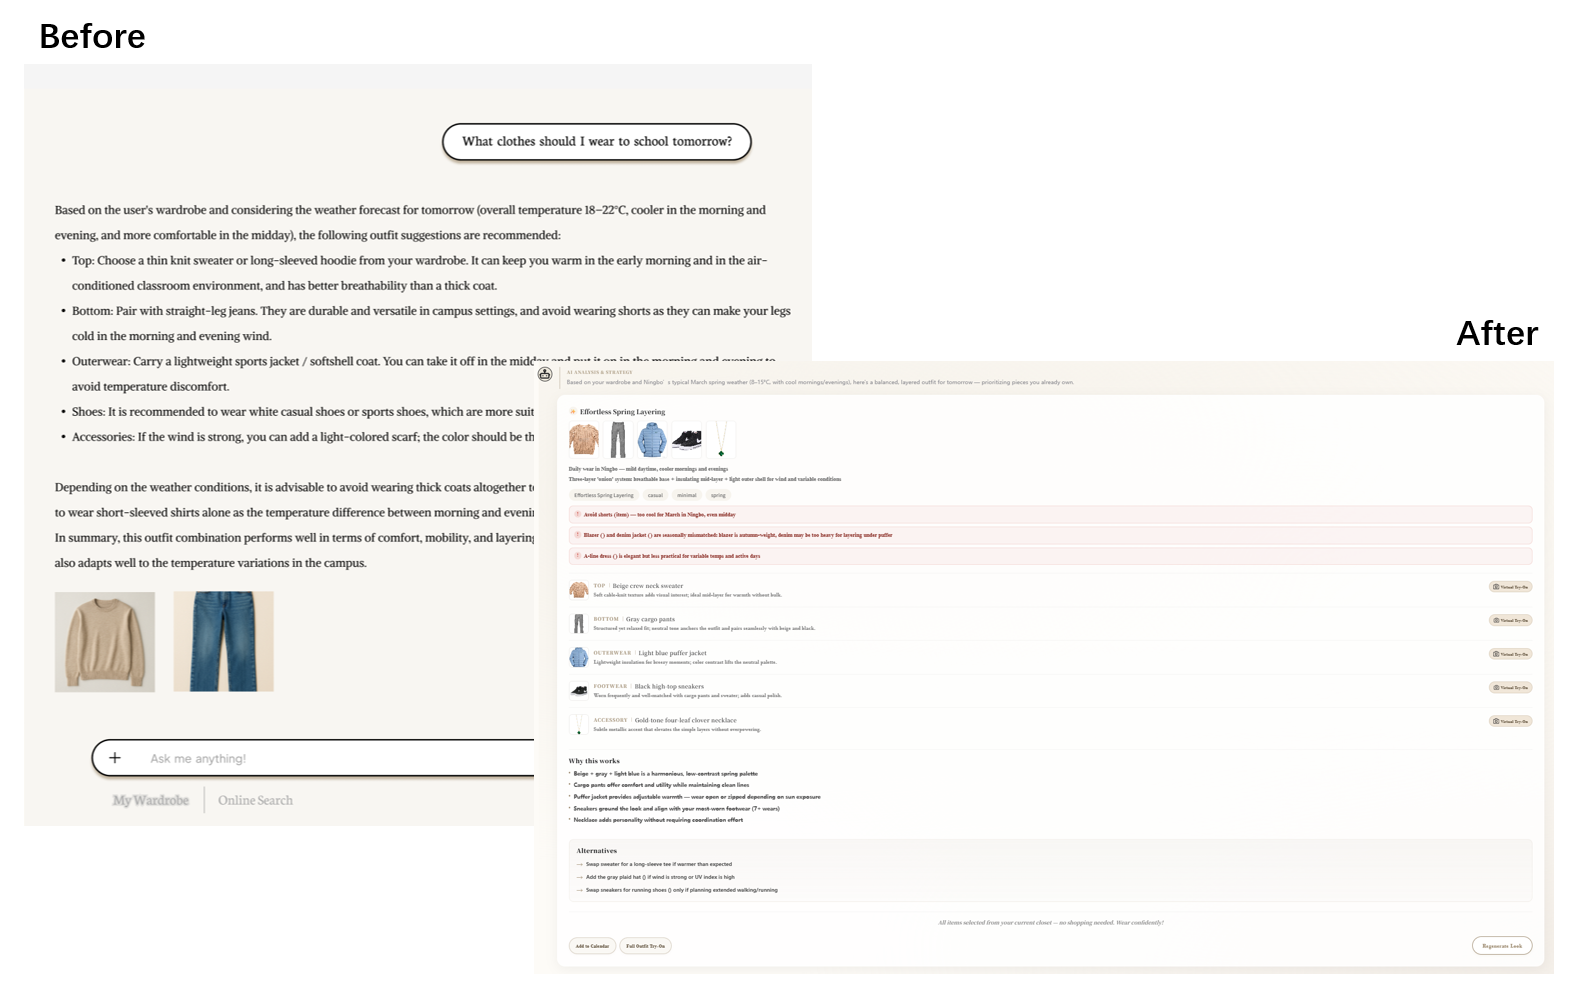
\includegraphics[width=0.8\textwidth]{images/Section_5/newUI/evolution/llm.png}
    \caption{Recommendation AI page evolution}
    \label{fig:LLM_evolution}
\end{figure}
In the initial design, the Recommendation AI module simply displayed generated text and images in a basic format. However, during implementation, it became clear that long LLM-generated responses were difficult to read and lacked structure. 

To address this issue, the output format of the LLM was constrained, and we introduced a structured UI rendering strategy. Instead of displaying plain text, the interface now distinguishes between different response types (e.g. recommendations and outfit plans), which significantly improves readability and interaction clarity.\\


\textbf{(2) Virtual Try-On module}

\begin{figure}[H]
    \centering
    
\includegraphics[width=0.8\textwidth]{images/Section_5/newUI/evolution/VTO.png}
    \caption{Virtual try-on page evolution}
    \label{fig:VTO_evolution}
\end{figure}
The original design placed uploaded images and generated results on a single page. However, this layout was not effective, as clothing images, full-body photos, and generated outputs are all vertically oriented. Displaying them together made each image appear too small. 

Therefore, the layout was redesigned to support vertical scrolling, with the default view focusing on the upload area. This change allows users to view content more clearly while maintaining a cleaner interface.\\


\textbf{(3) Calendar module}
\begin{figure}[H]
    \centering
    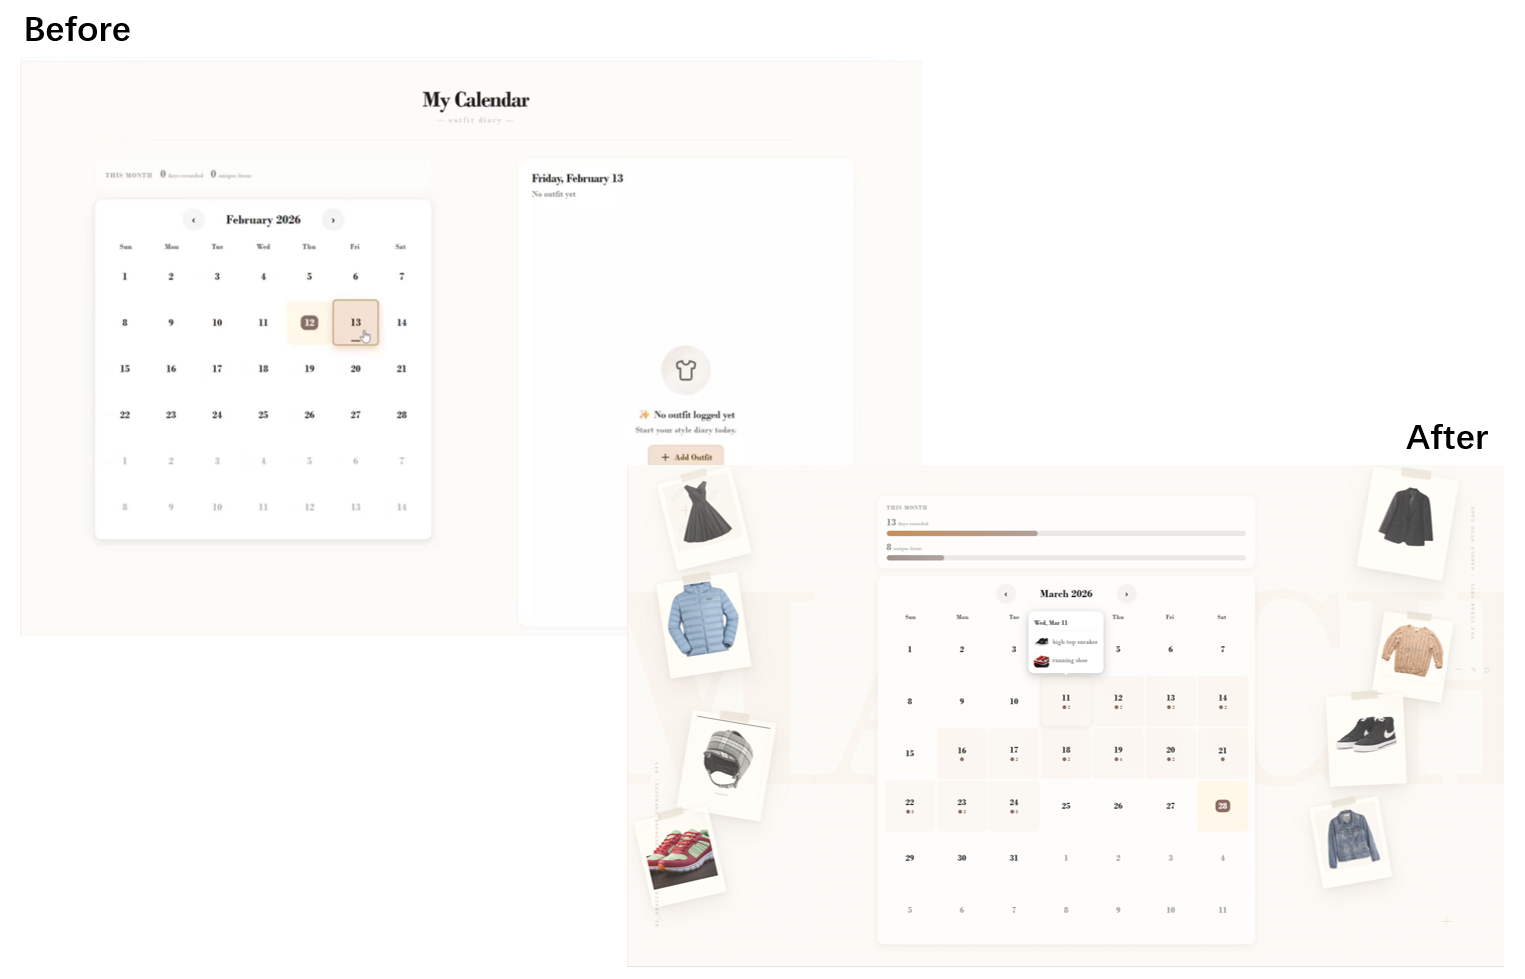
\includegraphics[width=0.8\textwidth]{images/Section_5/newUI/evolution/calendar.png}
    \caption{My Calendar page evolution}
    \label{fig:calendar_evolution}
\end{figure}
Initially, the calendar page was designed with a fixed layout, where the calendar was placed on the left and a detail panel on the right. However, this structure resulted in a poor user experience, as the interface felt crowded. 

To improve this, the layout was redesigned to make the calendar the main focus of the page. A polaroid-style photo wall was introduced as a dynamic background, displaying outfits from the current month. The detail panel is now only shown when a specific date is selected, which simplifies the interface and enhances user interaction.\\


Overall, these design changes were introduced to address practical usability issues encountered during development. As a result, our UI provides a more intuitive and visually clear user experience compared to the initial prototype.